% main.tex -- Paper 2, Elsevier Information Fusion (research article), elsarticle template.
% Status: outcome-independent parts drafted on 2026-10-28; no GATE result exists yet.
% Layout option: the Guide for Authors does not name the elsarticle option and measures pages on the final template.
% "preprint,12pt" is the single-column review layout; switch to "5p,twocolumn" to estimate the final page count (limit 35).
\documentclass[preprint,12pt]{elsarticle}

\usepackage{amsmath,amssymb,amsthm}
\usepackage{booktabs}
\usepackage{graphicx}
\usepackage{xcolor}
\usepackage[ruled,vlined,linesnumbered]{algorithm2e}
\usepackage{microtype}
\usepackage{seqsplit}
\emergencystretch=3em
\usepackage{hyperref}

% ---- project macros ---------------------------------------------------------------------------
% \todo marks every open fact. [AUTHOR: ...] = a fact only the authors can supply; [RESULT: ...] = a place for a result
% that does not exist yet. All \todo items must be resolved or deleted before submission.
\newcommand{\todo}[1]{{\color{red}\textbf{[#1]}}}
\newcommand{\mask}{\mathsf{M}}
\newcommand{\E}{\mathbb{E}}
\newcommand{\PP}{\mathbb{P}}
\newcommand{\ind}{\mathbb{1}}
\newcommand{\Var}{\mathrm{Var}}
\newcommand{\fp}{\texttt{fp32}}

\SetKwInOut{Input}{Input}\SetKwInOut{Output}{Output}\SetKwInOut{Data}{Data}
\SetKwProg{Fn}{Function}{:}{}
\SetKwComment{Comment}{$\triangleright$\ }{}

\theoremstyle{plain}
\newtheorem{proposition}{Proposition}
\theoremstyle{definition}
\newtheorem{remark}{Remark}

\journal{Information Fusion}

\begin{document}

\begin{frontmatter}

% Title is provisional and written last. It carries the scope (one model) and makes no fusion, repair or improvement claim
% (red-team condition C4).
\title{Calibrated gating of corrupted input tokens in a pretrained text-image masked diffusion model: a preregistered measurement on UniDisc}

\author[vit]{Shlok Kumar Goenka}
\author[vit]{[AUTHOR: supervising professor, full name]}
\affiliation[vit]{organization={[AUTHOR: school or department], Vellore Institute of Technology},
            city={Vellore},
            postcode={[AUTHOR: postcode]},
            state={Tamil Nadu},
            country={India}}
\cortext[cor]{[AUTHOR: corresponding author, postal address and published e-mail]}

\begin{abstract}
% Provisional abstract, at most 250 words once the \todo items are filled. No citations, no fusion or repair claim (C4).
% Every sentence about a result waits for the frozen run files.
A unified masked diffusion model treats every observed token as certain, although the tokens of a real input can be damaged
by compression, noise, splicing or a mismatched caption.
This paper asks whether a pretrained model can find damaged image tokens itself, and whether withholding them changes a
caption-verification decision.
Each image token is scored by its masked likelihood inside the image with the caption withheld.
A threshold is set by conformal risk control on clean image-caption pairs, so that the expected proportion of clean
tokens flagged is at most a chosen level.
Flagged tokens are removed from an additive image-to-caption evidence statistic.
The measurement is preregistered, runs on one pretrained 1.4B model with no network finetuning, and compares the gate
with no gate, with random masks of the same size and shape, with cheap non-generative detectors and with a pixel denoiser.
\todo{RESULT: headroom outcome (which corruptions leave room for a gate), realised false-alarm proportion with interval,
primary paired contrast per corruption with interval and Holm-adjusted p-value, mechanism and detection controls. Use only
the wording allowed by the preregistration, section 12; one sentence on scope: one model, one dataset.}
\end{abstract}

\begin{highlights}
% 3 to 5 items, at most 85 characters each; the working copy is highlights.txt. No fusion or repair claim (C4).
\item \todo{RESULT: see highlights.txt; written after the results are frozen}
\end{highlights}

\begin{keyword}
Masked discrete diffusion \sep Conformal risk control \sep Input reliability \sep False-alarm control \sep Vision-language tokens \sep Fault detection
% [AUTHOR: whether to add "Multimodal fusion" as a keyword is open (scope-fit decision M7); it is kept out until decided.]
\end{keyword}

\end{frontmatter}

\section{Introduction}\label{sec:intro}
% introduction.tex -- card v4 scope (eleven test families; P is the only headline family, SAP Addendum A4 Part 2 binds the wording of
% the contribution list). Drafted outcome-neutral on 2026-10-28; on 2026-10-29 the contribution list was completed for the label NEG
% of P (A4.2.4 items 3 and 5). Measured results quoted: the detection table of run P2-GATE-M1 (secondary family S-D, wording of
% decision D0074), the label sentence of P and the clean false-alarm check (run P2-GATE-M4).
% Must-not-claim list (NOVELTY-REAUDIT-GATE section 7; NOVELTY-CHECK-INFFUS section 4, items 10 to 13) is respected: no "first" claim,
% no "decision-level" for the gate, no sentence about Zhou and Lu that only their full text could support.

Input-token gating asks which of the observed tokens given to a model should be withheld before the model reasons from
them.
The question arises for any model that reads a sequence of discrete tokens as evidence, and it is sharp for masked
discrete diffusion models.
A masked diffusion model is trained to predict any masked token from any visible subset of the sequence, and the mask
token means ``unknown''~\cite{austin2021d3pm,sahoo2024mdlm,ou2025radd}.
Every token that is visible is therefore treated as certain.
This is acceptable for a clean training sequence.
It is a weakness when the input comes from a pipeline that compresses, adds noise to, crops, splices or mislabels the data,
because a single wrong visible token is used with the same confidence as a correct one.
Unified models extend the setting to two or more modalities in one token sequence~\cite{swerdlow2025unidisc,yang2025mmada,li2025lavida,shi2025muddit}.
In such a model a damaged image token can change what the model concludes about a caption, and the reverse.

\paragraph{Why this is a fusion problem.}
Each image token and each caption token is a source that reports a value, and the model combines them.
The paired decision studied here, whether a caption describes an image, sums per-token log-likelihood ratios over the 1\,024
image tokens of one image.
That is the rule used to fuse local decisions in distributed detection, in which each source is weighted by its reliability
before a global threshold is applied~\cite{chair1986optimal,tenney1981detection}; it is optimal for sources that are independent
given the hypothesis, which image tokens are not, so here it is an approximation (Section~\ref{ssec:limits}).
Imperfect and spurious data are a first-order difficulty of multisensor fusion~\cite{khaleghi2013multisensor,vempaty2013byzantine},
a survey in this journal organises multimodal fusion on low-quality data into noisy, incomplete, imbalanced and quality-varying
settings~\cite{zhang2026lowquality}, and evidential fusion methods discount each modality by an estimated
reliability~\cite{shao2024ddef,huang2025evidential}.
Classical practice also checks each source for a fault and isolates the faulty ones before fusing~\cite{willsky1976survey,gao2015survey},
and sets the detection threshold from clean data so that the false-alarm rate stays at a chosen value, as in constant false-alarm
rate (CFAR) detection~\cite{finn1968adaptive,rohling1983cfar}.
Here the image tokens are the sources, the masked denoiser is the model of what a healthy source looks like, and the gate is the
fault detector that runs before the evidence is summed.
We call this input-level source validation: the gate acts on the sources before the evidence sum, not on the output decision.
The paper proposes no new fusion rule; it specifies a gate, a threshold with a stated guarantee, and a preregistered measurement
of whether withholding the flagged tokens changes the decision.

\paragraph{A measured failure case.}
The gate helps only if the model's own masked likelihood separates damaged tokens from intact ones, and a detection measurement
made before the main test shows that it does so for one kind of damage and not for another.
% run: P2-GATE-M1
Tokens replaced by uniform random codes are separated almost perfectly (mean per-item AUROC 0.961 for a replaced patch and 0.955
for swapped codes), whereas the score is close to chance on JPEG compression (0.561) and Gaussian noise (0.503), where the changed
codes depend on the image content.
This is a measurement of the score in a secondary family (S-D, Section~\ref{ssec:res_det}); it does not enter the headline test and
is not used to interpret it.

\paragraph{What exists and what is missing.}
Many recent methods remask tokens in a masked diffusion model.
Most act on tokens that the sampler itself produced: they remask low-confidence commitments, learn a quality score, or
perturb the context to find brittle tokens
\cite{wang2025remdm,kim2025prism,schiff2026proseco,huang2025remedi,zhai2026core,yao2026remask,lezama2022tokencritic}.
In multimodal masked diffusion models the same idea has been applied to the model's own generations, with cross-modal
confidence as the trigger~\cite{ouyang2026freecorrection,le2026co2jump}.
Work on corrupted \emph{input} tokens is thinner.
Trust but Verify~\cite{jhingran2026trustverify} detects corrupted conditioning tokens in a text-only masked diffusion model,
re-noises them to the mask state and refills them; it needs a finetune, uses a hand-set threshold, and has no second modality.
Conformal risk control has been used with masking-derived scores to flag erroneous caption words given an image, with a
CLIP-based score and a threshold calibrated on labelled foil data~\cite{gomes2025crc}.
In this journal, Zhou and Lu~\cite{zhou2027burden} describe, in their abstract, a keep-or-override gate between two
vision-language recognisers whose threshold is chosen with a Clopper--Pearson bound on harmful overwrites; its unit is a whole
prediction rather than an input token.
The authors of UniDisc show repair of corrupted image-caption pairs by random masking and best-of-$n$ re-infilling in one
qualitative figure~\cite{swerdlow2025unidisc}.
Section~\ref{sec:related} gives the precise differences.
Three things are missing from this picture.
No measurement separates a gate that finds damaged tokens from a mask that merely has the same shape.
No threshold for input tokens carries a stated bound on the false-alarm proportion on clean inputs.
And no comparison shows whether withholding flagged tokens helps a cross-modal decision more than cheap non-generative
detectors or a pixel denoiser do.

\paragraph{Contributions, stated as a measurement.}
This paper does not claim to be the first to detect or remask corrupted input tokens, the first to remask in a unified
model, the first risk-controlled threshold for vision-language errors, or the first masked-likelihood or null-normalised
generative score.
The gate is the object of measurement here, not an asset whose merit is assumed.
Each numbered item corresponds to a result that the preregistered analysis delivered whatever it found.
\begin{enumerate}
\item \emph{The measured object} (Section~\ref{sec:method}). We specify an input-level source-validation gate for a pretrained
unified masked diffusion model: each image token is scored by the model's own masked likelihood with the caption withheld, and
the flag threshold is set by conformal risk control on clean pairs so that the expected flagged share of a clean pair's tokens is
at most $\alpha$.
\item \emph{A closed-form condition} (Section~\ref{ssec:evidence}). Under an independent-token approximation, we give the condition
on the false-alarm and hit rates under which discarding flagged tokens raises the signal-to-noise ratio of an additive evidence
sum; it is an approximation because image tokens are dependent, and it is not linked to any result of the primary test.
\item \emph{A preregistered test} (Sections~\ref{sec:protocol} and~\ref{ssec:res_primary}). An exact McNemar test with Holm
correction over three realistic corruptions, with the sample size fixed by a blind headroom rule, of whether withholding the
flagged tokens changes image-direction verification accuracy, with controls for mask geometry, texture and pixel denoising.
% A4.2.4 item 3, label NEG: the first clause of the opening of Section 6.1 (A4.2.3). run: P2-GATE-M4 (outcome.label = negative)
The preregistered test excludes an improvement or a loss of more than five percentage points in image-direction verification accuracy
from gating under JPEG quality~10, Gaussian noise with $\sigma=0.10$ and a $128$-pixel splice.
\item \emph{Token detection, measured} (Section~\ref{ssec:res_det}).
% run: P2-GATE-M1
At the token level the gate's score separates code-level random replacements (AUROC 0.961 for a patch, 0.955 for swapped codes)
but is near chance on JPEG and Gaussian noise (0.561 and 0.503).
On noise it is below a one-pass score without finetuning (0.607; the marginal 95\,\% intervals, 0.493--0.513 and 0.597--0.618, do
not overlap; no paired test was run), and on JPEG the two overlap (0.561, 0.547--0.575, against 0.581, 0.569--0.593).
In the preregistered comparison it is below a texture score whose sign was chosen on the same items (0.756 and 0.768), so the
preregistered falsifier for the score was met.
\item \emph{Calibration, checked} (Section~\ref{ssec:res_cal}). We check the clean false-alarm statement on held-out clean test
pairs.
% run: P2-GATE-M4 (calibration.fap_check.per_alpha.0.05)
At $\alpha=0.05$ the realised flagged share was 0.0456 (95\,\% interval 0.0442 to 0.0470), with no evidence of violation.
% A4.2.4 item 6: list only those of S2 and B whose status is "run, formal" or "run, descriptive", with that status; omit the item if
% neither ran. R was not run (gatekept: no primary rejection with b>c), so it is not listed.
\item \todo{RESULT (A4.2.4 item 6): \emph{Secondary families} (Sections~\ref{ssec:res_s2} and~\ref{ssec:res_text}): name only those
of re-infilling (S2) and two-way fusion on hard negatives (B) that ran, with their status; delete this item if neither ran.}
\end{enumerate}
The scope is one pretrained 1.4B model, one image-caption dataset, three realistic image corruptions in the primary family and
two sanity corruptions in a separate positive control (PS).
The primary endpoint is the image-direction statistic, which has headroom on clean pairs; the text direction is near ceiling
there, and Section~\ref{ssec:task} states what this choice limits.
Caption corruption is not tested.

\todo{AUTHOR: Figure 1 (motivation, page 1-2 per IF anatomy rule 31) is being prepared separately from committed run arrays; do not
draw it with a generative image tool.}

\paragraph{Roadmap.}
Section~\ref{sec:related} places the work against the closest methods.
Section~\ref{sec:method} defines the scores, the calibrated gate, the evidence statistic and the algorithms.
Section~\ref{sec:protocol} gives the data, folds, corruptions, arms, controls, the families and the reading of the primary test;
the preregistration record and the deviations are in \ref{app:prereg}.
Section~\ref{sec:results} reports the results family by family, Section~\ref{sec:discussion} discusses them with the limitations,
and Section~\ref{sec:conclusion} concludes.
\ref{app:timefree} gives the evidence that the model has no time input in the released configuration.


\section{Related work}\label{sec:related}
% related.tex -- sources: research/paper2/related/CLOSEST-WORK-2026-10-28.md, TRUST-BUT-VERIFY-READ-2026-10-28.md,
% REFERENCES-DRAFT-2026-10-28.md, NOVELTY-REAUDIT-GATE-2026-10-28.md. Descriptions of other papers stay at the level the
% reference notes support (abstract, or passage read); anything weaker is not stated.

The related work is organised along four axes: which tokens are treated as suspect, how a token is scored, how the
threshold is set, and what is done with a flagged token.
Table~\ref{tab:related} lists the closest works on these axes.

\paragraph{Masked diffusion and unified models.}
Absorbing-state discrete diffusion~\cite{austin2021d3pm,lou2024sedd} was simplified into masked diffusion language models
\cite{sahoo2024mdlm} and scaled~\cite{nie2025llada}.
A masked diffusion denoiser models the conditional distribution of a clean token given the unmasked context~\cite{ou2025radd},
which is the property the gate score uses.
Masked image-token generation~\cite{chang2022maskgit} and unified text-image models~\cite{swerdlow2025unidisc,yang2025mmada,li2025lavida,shi2025muddit}
put several modalities in one sequence.
UniDisc, the backbone used here, is trained to mask all tokens of a modality with some probability, so that a modality
likelihood with the other modality withheld exists~\cite{swerdlow2025unidisc}.
The appendix of that paper demonstrates repair of overlaid and mismatched image-caption pairs by random masking of both
modalities, re-unmasking and best-of-$n$ selection by the model's own likelihood, shown as examples without a metric or a
per-token score.
That recipe is the closest prior procedure for re-infilling and is treated as a baseline in Section~\ref{sec:protocol}.

\paragraph{Remasking and self-correction of generated tokens.}
Training-free remasking acts on the sampler's own commitments~\cite{wang2025remdm,zhai2026core,yao2026remask}.
Learned variants add a per-token quality score or a correction head~\cite{kim2025prism,schiff2026proseco,huang2025remedi}.
For masked image generation, a learned critic decides which sampled image tokens to resample~\cite{lezama2022tokencritic}.
In multimodal masked diffusion models, self-correction re-evaluates committed tokens with the token remasked and remasks the
lowest-scoring ones~\cite{ouyang2026freecorrection}.
A coupled sampler for concurrent text and image generation retracts commitments when cross-modal evidence turns against
them~\cite{le2026co2jump}.
All of these act on tokens that the model produced.
The tokens studied here are given evidence whose provenance is untrusted, which raises a question that does not arise for
self-correction: whether a suspect token should be withheld (left masked) or imputed (re-infilled).
The loop of detecting, remasking and refilling is not claimed as new, and the cross-modal remasking trigger belongs to the
works above.

\paragraph{Corrupted input and conditioning tokens.}
Trust but Verify~\cite{jhingran2026trustverify} is the nearest work.
It studies corrupted context tokens in a masked diffusion language model with 170M parameters, finetuned with substituted
context tokens.
Its suspicion score is the model's probability of the observed token at its unmasked position, its threshold is annealed
by hand within an edit budget derived from an assumed corruption rate, and flagged tokens are re-noised to the mask state and
refilled.
The paper reports a false-edit rate on clean tokens, and it reports that corruptions that are plausible under the left
context are only partly detected even with the finetune.
The present work differs in five ways: no finetuning of the network, a score computed after masking the token, with the
other modality withheld, a second modality, a threshold with a stated bound on the clean false-alarm proportion, and an outcome
measured on a cross-modal decision rather than on infilling quality.
Its observation that detection of plausible corruptions is hard is treated here as an expected difficulty for JPEG and noise,
with a stated falsifier (Section~\ref{sec:protocol}).
That paper also suggests that bidirectional consistency checking is needed for plausible corruptions; the masked score used
here is one way to make that check.
Because the finetune is what makes the observed-position probability informative in that paper, the baseline named
``TbV-score (non-finetuned)'' below reproduces its score but not its method.

In vision-language models, uncertainty-guided dropout decoding masks visual tokens that are uncertain under a
logit-lens projection, with hand-set drop probabilities and without a calibrated threshold~\cite{fang2025dropout}.
A self-purification defence masks visual tokens of high saliency at inference to remove backdoor behaviour~\cite{wan2026disp}.
Neither evaluates detection of corrupted tokens against known labels.

\paragraph{Masked-likelihood scores, null-normalised scores and calibrated thresholds.}
Scoring a token by its masked likelihood has a long history in text: the pseudo-log-likelihood~\cite{salazar2020mlm}, its
variant for multi-piece words~\cite{kauf2023plwl2r}, and unsupervised spelling detection from the probability of the original
token under a masked language model~\cite{li2022uchecker}.
A generative model can be used for image-text matching by normalising the conditional error with the unconditional one
\cite{krojer2023diffusionitm}, a null-normalised score that the pointwise-mutual-information statistics of this paper
resemble.
None of these is claimed as new.
Conformal prediction supplies distribution-free guarantees under exchangeability~\cite{vovk2005algorithmic,angelopoulos2023gentle},
conformal p-values give false-discovery control for outlier detection~\cite{bates2023outliers}, and conformal risk control
bounds the expected value of a monotone loss~\cite{angelopoulos2024crc}.
Gomes et al.~\cite{gomes2025crc} apply conformal risk control with masking-derived CLIPScore distributions to flag erroneous
caption words.
Their guarantee is a high-probability upper bound (Hoeffding and Bentkus) calibrated on foil-labelled data, with a CLIP
score that changes when words or patches are masked.
The calibration here uses clean pairs only, bounds an expectation, nests token losses inside items, and scores tokens
with a generative within-modality likelihood, including image tokens.
It does not make the guarantee of Gomes et al.\ the first of its kind, and it is not a stronger one: the two answer
different questions.

\begin{table}[t]
\centering
\caption{Closest works on the four axes of Section~\ref{sec:related}. Entries restate what the cited papers report, at the
level of detail read for this study; ``--'' means not applicable. AR: autoregressive. FAP: false-alarm proportion.}
\label{tab:related}
\footnotesize
\setlength{\tabcolsep}{3pt}
\begin{tabular}{p{0.18\linewidth}p{0.15\linewidth}p{0.22\linewidth}p{0.19\linewidth}p{0.14\linewidth}}
\toprule
Work & Tokens treated as suspect & Score & Threshold & Use of flagged tokens \\
\midrule
Trust but Verify \cite{jhingran2026trustverify} & Corrupted context tokens, text only & Probability of the observed token at its unmasked position (finetuned 170M model) & Hand-annealed, edit budget from an assumed rate; no guarantee & Re-noise to mask, refill \\
Gomes et al.~\cite{gomes2025crc} & Caption words given an image & Change of CLIPScore under masking & Conformal risk control, high-probability bound, foil-labelled calibration & Flag only \\
CO2Jump \cite{le2026co2jump} & Tokens generated by the sampler & Self-confidence and a cross-modal confidence term & Per-step quota from the schedule & Remask, resample \\
FreeCorrection \cite{ouyang2026freecorrection} & Tokens committed by the sampler & Likelihood of the committed token with it remasked & Lowest scores per step, schedule tuned on a validation set & Remask, resample \\
UniDisc, repair demo~\cite{swerdlow2025unidisc} & Random positions & -- & -- & Random mask, re-unmask, best of $n$ by model likelihood \\
Dropout decoding~\cite{fang2025dropout} & Visual tokens in an AR vision-language model & Divergence of a logit-lens distribution from the image mean & Hand-set drop probabilities & Drop in several masks, vote \\
\midrule
This paper & Input image tokens of a given pair & Masked likelihood in own modality, other modality withheld, normalised by the position marginal & Conformal risk control on clean pairs, expected FAP at most $\alpha$ & Withhold (marginalise) or re-infill \\
\bottomrule
\end{tabular}
\end{table}

\paragraph{Source validation before fusion.}
The classical background is outside machine learning.
Failure detection and isolation~\cite{willsky1976survey,gao2015survey}, CFAR thresholding~\cite{finn1968adaptive,rohling1983cfar,diao2024radar},
and decision fusion with weighted reliabilities~\cite{chair1986optimal,kittler1998combining} are the vocabulary the method
borrows.
Selecting the set of tokens to keep by looking at their values makes the missingness informative~\cite{rubin1976inference};
Section~\ref{sec:method} states the conditions under which withholding a data-selected set is still the right treatment.


\section{Method}\label{sec:method}
% method.tex -- source: research/paper2/method/GATE-METHOD-SPEC-v2-2026-10-28.md (v1 where v2 says unchanged).
% The only empirical numbers in this file are the M1 detection values quoted in Section "gate statistic" (run P2-GATE-M1, K2 wording).
% The only guarantee stated is the one the SAP (section 6) allows.
% Notation: symbols follow the SAP and exp_p2/gate/theory.py. Four letters with a second meaning were disambiguated in this revision
% (groups Gamma_k, sample count n_draw, empirical calibration risk F_cal, SNR flag probabilities phi_0, phi_1); crosswalk in Appendix A.
% Propositions: Prop. 1 (calibration) is conformal risk control applied, not a contribution; the marginalisation property is
% the standard denoiser property, not a contribution (must-not-claim items 5 and 6).
% Prop. 2 (correlated-token gating) is theory (D0078, D0079); it is never used to explain an E-pred result; Props. 1 and 3 of the theory addendum are not used here.

This section defines the notation, the scores, the calibrated gate, the evidence statistic and seven algorithms.
Each algorithm calls the earlier ones, and Algorithm~\ref{alg:gate} composes all of them.
The method has three steps.
Each input token is \emph{scored} by its masked log-likelihood inside its own modality with the other modality withheld.
Tokens whose score is improbable for clean inputs, at a threshold set on clean data, are \emph{gated}.
The decision then \emph{fuses} evidence from the tokens that remain (GATE-M, the marginalise arm), or from tokens re-infilled by
the model (GATE-I, the impute arm; the SAP calls it I-GATE).
Cost is counted in network passes, listed per quantity in \ref{app:diag}.
One design rule organises the three steps: evidence that is tested must not be used to gate (Section~\ref{ssec:separation}).
The denoiser is used through one conditional only, the probability of a token given a visible subset, called with no time
input; Section~\ref{ssec:data} and \ref{app:timefree} state what is checked about that property for the released
checkpoint.

\subsection{Setting and notation}\label{ssec:notation}
A unified masked discrete diffusion model with absorbing-state masking is given a sequence of caption tokens and image tokens.
The network $p_\theta$ maps a partly masked sequence to a categorical distribution at every masked position.
A pair is $x=(t,v)$ with caption tokens $t=(t_1,\dots,t_n)$ and image tokens $v=(v_1,\dots,v_m)$.
The modalities are $a,b\in\{T,I\}$ with $a\neq b$.
Table~\ref{tab:notation} lists the symbols.
All log-likelihoods are in nats, computed as an \fp{} log-softmax of the logits restricted to the vocabulary of the scored
modality.

\begin{table}[t]
\centering
\caption{Notation. Symbols follow the preregistration documents and the analysis code. A letter with a second use appears in a
separate row. Symbols used only in the protocol are defined there.}
\label{tab:notation}
\footnotesize
\begin{tabular}{p{0.27\linewidth}p{0.63\linewidth}}
\toprule
Symbol & Meaning \\
\midrule
$x=(t,v)$ & one pair of caption tokens $t$ ($n$ tokens) and image tokens $v$ ($m=1\,024$ tokens) \\
$\tilde x=(\tilde t,\tilde v)$, $v^\circ$ & the observed, possibly corrupted pair; the tokens of the clean image \\
$Z_j=\ind[\tilde v_j\neq v^\circ_j]$ & corrupted-token label (used only for evaluation) \\
$\mask$, $\varnothing^a$ & the mask token ($\mask$ means ``unknown''); all tokens of modality $a$ masked \\
$a,b\in\{T,I\}$ & scored modality and the other modality (text, image) \\
$p_\theta(x_j=\cdot\mid\cdot)$ & categorical of the network at masked position $j$ \\
$\Pi_K=\{\Gamma_1,\dots,\Gamma_K\}$ & random partition of the positions of modality $a$ into $K$ complementary groups; $k(j)$ is the group of $j$ \\
$A_j,B_j,C_j,D_j$ & four context levels of Eq.~\eqref{eq:levels}; $D_j[y]$ is the vector over codes $y$ and $D_j=D_j[x_j]$ \\
$q_j$, $u_j$ & hypothesis-free intra-modal evidence $B_j-D_j$ and suspicion $u_j=-q_j$ \\
$\alpha$, $\hat\tau$, $\widehat F_{\rm cal}$ & target false-alarm level, calibrated threshold, empirical calibration risk (Eq.~\ref{eq:crc}) \\
$G$, $R$ & gated (flagged) set and reliable set, the complement of $G$ \\
$c$, $c^+$, $c^-$ & a candidate caption, the true caption and a wrong caption \\
$\Lambda^c_j[y]$ & log-probability of image code $y$ at position $j$ with the image fully masked and caption $c$ visible \\
$\Delta_j$, $\bar\Delta_R$, $Y_R$ & per-token paired evidence, its mean over $R$, and the decision $\ind[\bar\Delta_R>0]$ (Eq.~\ref{eq:delta}) \\
$d_R$, $z_R$ & size-normalised evidence ratio and evidence $z$-score over $R$ (Eq.~\ref{eq:dz}) \\
$S_r$, $n_{\rm draw}$ & number of re-infill steps and of independent re-infill draws \\
$S$, $\rho$, $\mu,\sigma^2$, $\mu_c,\sigma^2_c$ & additive statistic $\sum_jI_j\Delta_j$; corrupted fraction; mean and variance of $\Delta_j$ on clean and on corrupted tokens (Eqs.~\ref{eq:mean}--\ref{eq:snr}) \\
$\phi_0$, $\phi_1$ & probability that a clean, respectively a corrupted, token is flagged in the signal-to-noise analysis; $\hat\phi_0,\hat\phi_1$ their observed values (called $\alpha$, $\beta$, $\alpha_{\rm obs}$, $\beta_{\rm obs}$ in the preregistration and the code) \\
$\gamma_0$, $\gamma_1$, $\gamma_{01}$ & correlation of $\Delta_j$ and $\Delta_k$, $j\neq k$, for two clean tokens, two corrupted tokens, and one of each (Proposition~\ref{prop:snrcorr}; theory only) \\
\bottomrule
\end{tabular}
\end{table}

\subsection{Masked scores}\label{ssec:scores}
For a token $j$ of modality $a$ with observed value $x_j$, four context levels are distinguished.
Let $\Gamma_{k(j)}$ be the group of $j$ in a partition $\Pi_K$, and let $x^a_{-\Gamma}$ denote the tokens of modality $a$ outside $\Gamma$.
\begin{align}
A_j &= \log p_\theta\big(x_j\mid x^a_{-\Gamma_{k(j)}},\,x^b\big), &
B_j &= \log p_\theta\big(x_j\mid x^a_{-\Gamma_{k(j)}},\,\varnothing^b\big),\notag\\
C_j &= \log p_\theta\big(x_j\mid \varnothing^a,\,x^b\big), &
D_j &= \log p_\theta\big(x_j\mid \varnothing^a,\,\varnothing^b\big).
\label{eq:levels}
\end{align}
$A_j$ uses the rest of the own modality and the other modality; $B_j$ uses the own modality only; $C_j$ uses the other
modality only; $D_j$ uses nothing and is the position marginal.
By subtraction, the total pointwise mutual information splits in two ways,
\begin{align}
A_j-D_j&=\underbrace{(B_j-D_j)}_{q_j:\ \text{intra-modal}}+\underbrace{(A_j-B_j)}_{\text{cross-modal given own context}}\notag\\
&=\underbrace{(A_j-C_j)}_{\text{intra-modal given }b}+\underbrace{(C_j-D_j)}_{\text{cross-modal}}.
\label{eq:pmi}
\end{align}
The quantity $q_j=B_j-D_j$ asks whether token $j$ is consistent with the rest of its own modality, relative to how likely
the value is at that position anyway.
It never sees the other modality, and therefore never sees the hypothesis that will be tested.
The cross-modal term $C_j-D_j$ is the decision evidence.
All four levels come from one primitive, Algorithm~\ref{alg:maskedscore}.

\begin{algorithm}[t]
\caption{\textsc{MaskedScore}: log-likelihood of target tokens under a mask pattern}\label{alg:maskedscore}
\Input{sequence $x$; target positions $P$; extra masked positions $X$; vocabulary slice $[lo,hi)$ of the targets}
\Output{$\lambda_j=\log p_\theta(x_j\mid\cdot)$ and $\pi^{\max}_j=\max_y p_\theta(y\mid\cdot)$ for $j\in P$}
\Fn{\textsc{MaskedScore}$(x,P,X,[lo,hi))$}{
  $\tilde x\leftarrow x$; set $\tilde x_P\leftarrow\mask$ and $\tilde x_X\leftarrow\mask$\;
  $\ell\leftarrow$ logits of $\tilde x$ \Comment*[r]{one network pass; batched with others}
  \For{$j\in P$}{
    $\eta_j\leftarrow\mathrm{logsoftmax}_{\fp}\big(\ell_{j,[lo,hi)}\big)$\;
    $\lambda_j\leftarrow\eta_j[x_j-lo]$ and $\pi^{\max}_j\leftarrow\exp\max\eta_j$\;
  }
  \Return $(\lambda,\pi^{\max})$\;
}
\end{algorithm}

\subsection{The gate statistic and the evidence-separation rule}\label{ssec:separation}
Two regimes are fixed per task before any run.
In the regime with \emph{no trusted reference} (detection, verification, matching), neither modality may be used to judge
the other, because the cross-modal relation is what is being tested.
In the regime with a \emph{trusted reference} (repair with a known clean caption), the trusted modality may be used in the gate,
as a predicted state is used in an innovation gate of tracking.
The paper studies the first regime.

\emph{Evidence-separation rule:} in the first regime, the gate may use only statistics computed with the other modality
masked, that is $B_j$ and $D_j$.
A gate that used $A_j$ with a candidate caption visible would give each candidate a different evidence set, and a gate that removed
low cross-modal-evidence caption words would remove exactly the words that make a wrong caption wrong.
The gate statistic is therefore
\begin{equation}
u_j=-q_j=-(B_j-D_j),
\label{eq:suspicion}
\end{equation}
where a larger $u_j$ means a more suspicious token.
The division by the position marginal $D_j$ is the optimal normalisation in one idealised case only: if a corrupted value is
drawn from the model's own position marginal independently of context, $q_j$ is the Neyman--Pearson statistic, whereas for
a uniform alternative, that is for corruptions that replace tokens by uniform random codes, the plain likelihood $B_j$ is.
Neither case is assumed to hold for JPEG, noise or splice, whose changed codes depend on the content, and no proposition about
detection power is claimed for them.
The null normalisation is therefore not assumed to improve detection, and the measurement does not show that it does.
% run: P2-GATE-M1
On the two uniform-code corruptions plain-$B$ has a slightly higher mean per-item AUROC than $q$ (patch 0.964 against 0.961,
swap 0.960 against 0.955), and on JPEG and noise the two differ by less than 0.01 (0.560 against 0.561, and 0.511 against 0.503;
no paired test was run on these two corruptions); Section~\ref{ssec:res_det} reports the full table.
Detection of content-dependent damage is an empirical question (Section~\ref{sec:protocol}).
The score $A_j-B_j$ without the null term cancels the own-context surprise of a corrupted token, because the term appears in
both $A_j$ and $B_j$; it is kept only as a control.

On the text side the gating unit is a word, that is a word-initial piece and its continuation pieces, and the suspicion of a
word is the maximum of the suspicions of its pieces (equivalently, the minimum of their $q$), following the idea that
multi-piece words need a word-level score~\cite{kauf2023plwl2r}.
Gating a word masks all its pieces.

\begin{algorithm}[t]
\caption{\textsc{ReliabilityScores}: suspicion of every token of one modality}\label{alg:reliability}
\Input{observed pair $\tilde x$; modality $a$; number of groups $K$; seed}
\Output{suspicion vector $u$ over the positions of $a$}
\Fn{\textsc{ReliabilityScores}$(\tilde x,a,K,\mathrm{seed})$}{
  draw a partition $\Pi_K$ of the positions of $a$ from the seed\;
  \For{$k=1,\dots,K$}{
    $B_{\Gamma_k}\leftarrow$ \textsc{MaskedScore}$(\tilde x,\ \Gamma_k,\ \text{positions of }b,\ \text{slice of }a)$ \Comment*[r]{$b$ withheld}
  }
  $D\leftarrow$ \textsc{MaskedScore}$(\tilde x,\ \text{all of }a,\ \text{all of }b,\ \text{slice of }a)$ \Comment*[r]{layout only; cached}
  $u_j\leftarrow-(B_j-D_j)$ for every position $j$ of $a$\;
  \lIf{$a=T$}{aggregate $u$ to words by the maximum over the pieces of a word}
  \Return $u$\;
}
\end{algorithm}

\subsection{Calibration by conformal risk control}\label{ssec:calibration}
The threshold is set on a calibration set $\mathcal D_{\rm cal}$ of $n_{\rm cal}$ clean pairs, disjoint by image from every other fold.
``Clean'' means images as distributed in the data set and passed through the tokenizer; corruption labels are relative to
that tokenisation.
For item $i$ with $m_i$ gating units and suspicions $u_{ij}$, the false-alarm proportion at threshold $\tau$ is
\begin{equation}
L_i(\tau)=\frac1{m_i}\sum_{j=1}^{m_i}\ind\big[u_{ij}>\tau\big]\in[0,1],
\label{eq:loss}
\end{equation}
which is non-increasing in $\tau$.
Define the empirical calibration risk $\widehat F_{\rm cal}(\tau)=n_{\rm cal}^{-1}\sum_i L_i(\tau)$ and the threshold
\begin{equation}
\hat\tau=\inf\Big\{\tau:\ \frac{n_{\rm cal}}{n_{\rm cal}+1}\,\widehat F_{\rm cal}(\tau)+\frac1{n_{\rm cal}+1}\le\alpha\Big\},
\label{eq:crc}
\end{equation}
with $\hat\tau=+\infty$ if the set is empty, so that nothing is flagged.
A token is flagged when $u_{ij}>\hat\tau$ with a strict inequality.

\begin{proposition}[calibration guarantee; conformal risk control applied]\label{prop:crc}
Let the calibration items and a new clean test item be exchangeable as items, and let $L_i$ be defined by
Eq.~\eqref{eq:loss}, with scores that have no ties.
Then $\E\big[L_{\rm test}(\hat\tau)\big]\le\alpha$.
\end{proposition}
\noindent\emph{Proof.} The loss is bounded by one and non-increasing in the threshold, so the statement is Theorem~1 of
conformal risk control~\cite{angelopoulos2024crc} with bound $B=1$. \qed

\paragraph{Wording and scope of the guarantee.}
The statement made in this paper, and no stronger one, is: the threshold is calibrated so that, for a clean test pair
exchangeable with the calibration pairs, the expected proportion of its tokens that are flagged is at most $\alpha$.
Three details keep the statement true in practice.
The bound is over items, so tokens inside an item need not be exchangeable or independent and positions may have different
score distributions.
Ties, which arise from \texttt{bf16} logits, are broken by an independent uniform jitter $\epsilon\sim U(0,\epsilon_0)$ added to
calibration and test scores, with $\epsilon_0$ below the smallest non-zero gap between distinct calibration scores, computed
and not chosen.
The statistic, $K$, $\alpha$ and the fold sizes are fixed before any test item is scored, because choosing them from calibration
or test items would break exchangeability.
The guarantee is marginal over the draw of the calibration set, so one realised calibration set may lie above $\alpha$ on a
finite test set.

\paragraph{What is not guaranteed.}
There is no bound on detection power: calibration controls false alarms on clean items only.
There is no bound on false alarms among the clean tokens of a \emph{corrupted} item, whose neighbours see contaminated context
and can be flagged more often; that rate is measured and reported (Section~\ref{sec:protocol}).
There is no guarantee under shift between calibration and test, such as another data set, caption style, resolution or
tokenizer.
Iterating the gate by re-scoring after masking breaks monotonicity in $\tau$, so the bound would not apply to it.
Words such as ``certified'' or ``provably reliable'' are not used for this gate.

\begin{algorithm}[t]
\caption{\textsc{CalibrateThreshold}}\label{alg:calibrate}
\Input{calibration set $\mathcal D_{\rm cal}$; modality $a$; level $\alpha$; $K$; seed rule}
\Data{clean pairs only, disjoint from all other folds}
\Output{threshold $\hat\tau$ and jitter scale $\epsilon_0$, stored with the hash of the item list, $K$, seed and statistic name}
\Fn{\textsc{CalibrateThreshold}$(\mathcal D_{\rm cal},a,\alpha,K)$}{
  \For{each item $i$ in $\mathcal D_{\rm cal}$}{
    $u_i\leftarrow$ \textsc{ReliabilityScores}$(x_i,a,K,\mathrm{seed}_i)$\;
  }
  $\epsilon_0\leftarrow$ a value below the smallest non-zero gap between distinct pooled scores\;
  add independent jitter $\epsilon_{ij}\sim U(0,\epsilon_0)$ to every $u_{ij}$\;
  evaluate $\widehat F_{\rm cal}(\tau)$ at every distinct pooled value and return the smallest $\tau$ satisfying Eq.~\eqref{eq:crc}\;
}
\end{algorithm}

\subsection{Gating}\label{ssec:gate}
The gate applies the frozen threshold to the suspicions of an observed pair.
Algorithm~\ref{alg:gate_set} computes the gated set $G$ and the reliable set $R$ with the same $K$, seed rule and statistic as
in calibration.
No iteration is used.

\begin{algorithm}[t]
\caption{\textsc{Gate} (uses Algorithms~\ref{alg:reliability} and~\ref{alg:calibrate})}\label{alg:gate_set}
\Input{observed pair $\tilde x$; modality $a$; frozen $\hat\tau$ and $\epsilon_0$; $K$}
\Output{gated set $G$, reliable set $R$, suspicion $u$}
\Fn{\textsc{Gate}$(\tilde x,a,\hat\tau,\epsilon_0,K)$}{
  $u\leftarrow$ \textsc{ReliabilityScores}$(\tilde x,a,K,\mathrm{seed})$\;
  add independent jitter $\epsilon_j\sim U(0,\epsilon_0)$ to every $u_j$\;
  $G\leftarrow\{j:u_j>\hat\tau\}$; $R\leftarrow$ complement of $G$\;
  \Return $(G,R,u)$\;
}
\end{algorithm}

\subsection{Withholding flagged tokens: GATE-M (marginalise)}\label{ssec:marginalise}
Masking a flagged token tells the network that its value is unknown.
For a network that equals the Bayes-optimal denoiser of the absorbing-state objective, masking the set $G$ marginalises it:
for a masked target $j\notin G$,
\begin{equation}
p_\theta(x_j\mid x_R,\,x_G=\mask)=\sum_{x_G}p(x_j\mid x_R,x_G)\,p(x_G\mid x_R)=p(x_j\mid x_R).
\label{eq:marginalise}
\end{equation}
This is the standard property of such denoisers~\cite{ou2025radd}, not a contribution.
A real network approximates it.
Structured patterns, such as a contiguous block of masked image tokens together with a fully masked caption, are rare under
random per-token masking, so the amortisation error may be larger there; a coherence test on the real model is part of the
protocol (Section~\ref{sec:protocol}).

When the set $G$ is selected from the observed values, Eq.~\eqref{eq:marginalise} is not enough.
Let $Y$ be the quantity to infer, for example the caption hypothesis.
Using $p(Y\mid\tilde v_R)$ equals the Bayes answer under the corruption model when four conditions hold:
(i) $R$ contains no corrupted token;
(ii) corrupted values carry no information about the clean values, which holds for replacement by uniform random codes
and fails for JPEG and noise;
(iii) corruption locations are independent of the content, which fails where changed codes concentrate in regions in which the
tokenizer is unstable;
(iv) no clean token is in $G$, or the clean tokens in $G$ are uninformative about $Y$.
The gate selects on the observed values, so the missingness is informative~\cite{rubin1976inference}.
Each violation has a cost: residual corrupted evidence in (i), discarded signal in (ii) because a noisy copy would call for a
denoising posterior and not for marginalisation, a wrong distribution $p(v_G\mid v_R)$ for selected positions in (iii), and lost
clean evidence at rate $\alpha$ in (iv).
The conditions therefore favour withholding for corruptions that satisfy (ii) and (iii) and are least favourable, possibly
not at all, for JPEG and noise; this is stated in advance and is not an account of any result.

\subsection{Image-direction evidence}\label{ssec:evidence}
The decision studied is paired verification: for one image, does the true caption $c^+$ explain the image better than a wrong
caption $c^-$.
The image-direction evidence uses one pass per caption with all image tokens masked and the caption visible.
Let $\Lambda^c_j[y]$ be the log-probability of code $y$ at image position $j$ in that pass, so that
\begin{equation}
\Delta_j=\Lambda^{c^+}_j[\tilde v_j]-\Lambda^{c^-}_j[\tilde v_j],\qquad
\bar\Delta_R=\frac1{|R|}\sum_{j\in R}\Delta_j,\qquad
Y_R=\ind\big[\bar\Delta_R>0\big].
\label{eq:delta}
\end{equation}
The position marginal $D_j$ cancels in the difference for a fixed image, so $\Delta_j=(C_j(c^+)-D_j)-(C_j(c^-)-D_j)$.
For a single candidate the per-caption evidence is $E_{I\leftarrow T}(c)=|R|^{-1}\sum_{j\in R}\big(\Lambda^{c}_j[\tilde v_j]-D_j[\tilde v_j]\big)$, and
$\bar\Delta_R=E_{I\leftarrow T}(c^+)-E_{I\leftarrow T}(c^-)$.
The logits of this pass do not depend on the image, which enters only through the gathered entries.
Hence all arms that differ in the set $R$ (no gate, gate, random gates, a changed-code gate, a denoised copy) reuse the same two
passes per item.
Ties and an empty set count as wrong, $Y=0$.
Two continuous summaries are used in the secondary analyses,
\begin{equation}
d_R=\frac{\bar\Delta_R}{s_R},\qquad z_R=\sqrt{|R|}\,d_R,
\label{eq:dz}
\end{equation}
where $s_R$ is the sample standard deviation of $\Delta_j$ over $R$.
The ratio $d_R$ rises when tokens with extreme per-token evidence are removed for any reason, which is why a random gate and
an uncertainty-ranked gate of equal size are reported next to it.

\begin{algorithm}[t]
\caption{\textsc{ImageEvidence} (GATE-M; uses Algorithms~\ref{alg:maskedscore} and~\ref{alg:gate_set})}\label{alg:evidence}
\Input{observed image tokens $\tilde v$; candidate captions $c_1,\dots,c_N$; reliable set $R$ from \textsc{Gate} or another arm; cached position marginal $D$}
\Output{$E_{I\leftarrow T}(c_k)$ for every candidate and, for a pair $(c^+,c^-)$, the paired quantities $Y_R$, $\bar\Delta_R$, $d_R$}
\Fn{\textsc{ImageEvidence}$(\tilde v,\{c_k\},R)$}{
  \For{each candidate $c_k$}{
    $\Lambda^{c_k}\leftarrow$ \textsc{MaskedScore} with all image tokens masked and $c_k$ visible, keeping the \fp{} log-probabilities over all image codes at all $m$ positions\Comment*[r]{one pass; reusable by every arm}
    $E_{I\leftarrow T}(c_k)\leftarrow\frac1{|R|}\sum_{j\in R}\big(\Lambda^{c_k}_j[\tilde v_j]-D_j[\tilde v_j]\big)$\;
  }
  \lIf{$N=2$}{$\Delta_j\leftarrow\Lambda^{c^+}_j[\tilde v_j]-\Lambda^{c^-}_j[\tilde v_j]$ for $j\in R$; \Return $\big(\ind[\bar\Delta_R>0],\ \bar\Delta_R,\ \bar\Delta_R/s_R\big)$}
  \Return $\{E_{I\leftarrow T}(c_k)\}$\;
}
\end{algorithm}

\paragraph{Analysis: when does withholding help an additive statistic?}\label{par:snr}
Consider the statistic $S=\sum_j I_j\Delta_j$ over $m$ tokens, with $I_j\in\{0,1\}$ the indicator that token $j$ is kept.
Under an independent-token approximation, clean tokens have mean $\mu$ and variance $\sigma^2$ and are kept with probability
$1-\phi_0$, corrupted tokens have mean $\mu_c$ and variance $\sigma_c^2$ and are kept with probability $1-\phi_1$, and a fraction
$\rho$ of tokens is corrupted.
Then
\begin{align}
\E S&=m\big[(1-\rho)(1-\phi_0)\mu+\rho(1-\phi_1)\mu_c\big],\label{eq:mean}\\
\Var S&=m\Big[(1-\rho)\big\{(1-\phi_0)\sigma^2+\phi_0(1-\phi_0)\mu^2\big\}\notag\\
&\qquad+\rho\big\{(1-\phi_1)\sigma_c^2+\phi_1(1-\phi_1)\mu_c^2\big\}\Big].\label{eq:var}
\end{align}
The no-gate case is $\phi_0=\phi_1=0$, and the gate raises $\E S/\sqrt{\Var S}$ if the ratio after exceeds the ratio before.
For $\mu_c=0$ this reduces to
\begin{equation}
\rho\,\sigma_c^2\,(\phi_1-2\phi_0+\phi_0^2)\;>\;\phi_0(1-\phi_0)(1-\rho)\,(\sigma^2+\mu^2).
\label{eq:snr}
\end{equation}
Three consequences are stated in advance.
A necessary condition is $\phi_1>2\phi_0-\phi_0^2$.
A random gate has $\phi_1=\phi_0$, for which the left side is negative, so it lowers the ratio.
On a clean item ($\rho=0$) any gate with $\phi_0>0$ lowers the ratio slightly.
The model is an approximation, since neighbouring tokens are correlated, and $\mu_c$ need not be zero even for random codes: a
caption that makes the predicted image distribution flatter gives random codes a higher probability.
The protocol estimates $\rho,\mu,\sigma^2,\mu_c,\sigma_c^2$ and the observed flag rates $\hat\phi_0,\hat\phi_1$ per corruption from
the per-token terms, and reports in how many corruptions the sign of the plug-in change of the ratio agrees with the sign of the
observed net accuracy difference (descriptive family E-pred, Section~\ref{ssec:families}); it is not a test and enters no claim
about the primary result.
E-pred uses Eqs.~\eqref{eq:mean}--\eqref{eq:var} as committed, and Proposition~\ref{prop:snrcorr} below is neither used by it nor
used to explain or interpret any E-pred result, agreeing or not.

\paragraph{Correlated tokens.}\label{par:snrcorr}
Eqs.~\eqref{eq:mean}--\eqref{eq:snr} treat the per-token terms as independent, which is an approximation for image tokens.
The following statement replaces independence by an exchangeable correlation within and between the two classes of tokens.
It is theory under stated assumptions and is not evaluated on the model.
The new symbols are $\gamma_0$, $\gamma_1$ and $\gamma_{01}$, the correlations of two clean, two corrupted, and one clean and one
corrupted token.

\begin{proposition}[withholding with exchangeably correlated tokens]\label{prop:snrcorr}
Condition on the corruption labels, so that $(1-\rho)m$ tokens are clean and $\rho m$ are corrupted, with the moments
$\mu,\sigma^2,\mu_c,\sigma_c^2$ and the keep probabilities $1-\phi_0$, $1-\phi_1$ of Eqs.~\eqref{eq:mean}--\eqref{eq:var}.
Assume (a) that for $j\neq k$ the correlation of $\Delta_j$ and $\Delta_k$ is $\gamma_0$ if both tokens are clean, $\gamma_1$ if both
are corrupted and $\gamma_{01}$ otherwise, with values for which the covariance matrix is positive semi-definite; and (b) that the
keep indicators $I_j$ are independent of each other and of every $\Delta_k$.
Then $\E S$ is given by Eq.~\eqref{eq:mean}, and, under (a) and (b),
\begin{equation}
\begin{aligned}
\Var S={}&V+(1-\rho)m\big((1-\rho)m-1\big)(1-\phi_0)^2\gamma_0\sigma^2\\
&+\rho m(\rho m-1)(1-\phi_1)^2\gamma_1\sigma_c^2\\
&+2\rho(1-\rho)m^2(1-\phi_0)(1-\phi_1)\gamma_{01}\sigma\sigma_c,
\end{aligned}
\label{eq:varcorr}
\end{equation}
where $V$ is the right side of Eq.~\eqref{eq:var}.
If moreover $\mu_c=0$ and $\E S>0$ with and without the gate, the gate raises $\E S/\sqrt{\Var S}$ if and only if
\begin{equation}
\begin{aligned}
&\rho\,\sigma_c^2\Big[(\phi_1-2\phi_0+\phi_0^2)\\
&\qquad+(\rho m-1)\,\gamma_1\,(\phi_1-\phi_0)(2-\phi_0-\phi_1)\Big]\\
&\quad+2\rho(1-\rho)\,m\,\gamma_{01}\,\sigma\sigma_c\,(1-\phi_0)(\phi_1-\phi_0)\\
&\qquad>\;(1-\rho)\,\phi_0(1-\phi_0)\,(\sigma^2+\mu^2).
\end{aligned}
\label{eq:snrcorr}
\end{equation}
Consequently:
(i) $\gamma_0$ does not enter Eq.~\eqref{eq:snrcorr}, and at $\gamma_1=\gamma_{01}=0$ it is Eq.~\eqref{eq:snr};
(ii) a gate with $\phi_1=\phi_0$, such as a random gate, lowers the ratio for every admissible correlation, and if $\gamma_{01}\ge0$ every
gate with $\phi_1\le\phi_0$ lowers it;
(iii) where $\phi_1>\phi_0$, a larger $\gamma_1$ or $\gamma_{01}$ can only turn a decrease of the ratio into an increase, so positive
correlation among corrupted tokens, or between clean and corrupted tokens, enlarges the region of $(\phi_0,\phi_1)$ in which the gate
raises the ratio, and as $(\rho m-1)\gamma_1\to\infty$ that region tends to $\{\phi_1>\phi_0\}$;
(iv) if $\gamma_{01}<0$, a gate that flags only clean tokens can raise the ratio;
(v) unlike Eq.~\eqref{eq:snr}, the condition depends on $m$.
\end{proposition}

\noindent\emph{Proof sketch.} Each of the $m(m-1)$ ordered pairs of distinct tokens adds $\E I_j\,\E I_k\,\mathrm{Cov}(\Delta_j,\Delta_k)$
to $\Var S$, which gives the three correlation terms of Eq.~\eqref{eq:varcorr}.
With $\mu_c=0$ the gate multiplies $\E S$ by $1-\phi_0$, so it raises the ratio if and only if
$(1-\phi_0)^2\,\Var S|_{\phi_0=\phi_1=0}>\Var S$; the clean-pair terms scale by $(1-\phi_0)^2$ on both sides and cancel, and the
remaining terms, divided by $m$, give Eq.~\eqref{eq:snrcorr}.
Appendix~\ref{app:snrcorr} gives the full proof. \qed

At zero correlation the statement is the independent-token analysis above: Eq.~\eqref{eq:varcorr} reduces to Eq.~\eqref{eq:var} and
Eq.~\eqref{eq:snrcorr} to Eq.~\eqref{eq:snr}.
Correlation therefore moves the gating frontier in the way (ii)--(iv) state, and independence is an approximation whose effect on the
frontier is of that kind and not of a fixed sign.
The ratio in Proposition~\ref{prop:snrcorr} is the signal-to-noise ratio of the sum.
If the per-token terms are jointly Gaussian, the accuracy $P(S>0)$ given the flags is $\Phi$ of the conditional ratio, which the
unconditional ratio approximates; without joint Gaussianity no statement about accuracy follows, and a gate can raise the ratio while
lowering the accuracy.
Assumption (b) is an approximation for GATE, whose flags are computed from the same token values as the evidence.
With correlation the ratio no longer grows like $\sqrt m$: it tends to a limit set by the shared component of the per-token terms.

\subsection{Text-direction evidence and conditioning arms}\label{ssec:text}
The text direction scores the caption tokens given the image.
With caption $c$ fully masked and the image visible, the evidence is the sum over caption tokens of the log-probability minus the same pass with the image
masked,
\begin{equation}
E_{T\leftarrow I}(c)=\sum_{j}\big(C_j-D_j\big),
\label{eq:text}
\end{equation}
where the image tokens in the gated set $G$ are masked in the first pass.
This is a conditioning arm in which the network, and not the arithmetic of a sum, withholds the flagged tokens.
In the exploratory analyses the statistic is the mean per-token value.

\subsection{Re-infilling flagged tokens: GATE-I (impute)}\label{ssec:reinfill}
Instead of leaving flagged tokens masked, the model can fill them in.
Algorithm~\ref{alg:reinfill} samples $n_{\rm draw}$ completions in $S_r$ steps, unmasking at step $s$ the next $k_s$ positions
of a random order drawn up front, and keeps the draw with the highest chain log-likelihood under the model itself, with the
caption masked (best of $n_{\rm draw}$; GATE-I).
The sampler is unguided and samples each position from the softmax at temperature one; it is the sampler fixed in the analysis plan
and not the sampler of the backbone's authors.
A hybrid variant that keeps only filled values whose recorded probability reaches $\kappa$ is described in the specification
and is not part of any preregistered family.
If the filled tokens are generated with the candidate caption visible, the evidence for that caption is biased upward.
Writing $\hat v_G\sim p(v_G\mid v_R,c)$, Bayes' rule gives
\begin{align}
\E\big[\log p(c\mid v_R,\hat v_G)\big]&=\log p(c\mid v_R)+\mathrm{KL}\big(p(v_G\mid v_R,c)\,\|\,p(v_G\mid v_R)\big)\notag\\
&\ge\log p(c\mid v_R),
\label{eq:leak}
\end{align}
so every candidate receives a non-negative bonus equal to how strongly it constrains the filled region, which need not favour the
true caption.
The rule is therefore to re-infill with the caption masked and to run the caption-visible variant only as a leakage control.
With exact sampling from $p(v_G\mid v_R)$, the expectation of $p(c\mid v_R,\hat v_G)$ equals $p(c\mid v_R)$, so GATE-I
is unbiased for GATE-M in the probability domain; in the log domain an $n_{\rm draw}$-sample estimate is biased downward by
Jensen's inequality and adds sampling variance.
Marginalising and imputing are not compared as a test: the preregistered re-infill family S2 compares the repaired flagged set
with repairing an equal-size random set (Section~\ref{ssec:families}).

\begin{algorithm}[t]
\caption{\textsc{ReInfill} (GATE-I; uses Algorithms~\ref{alg:maskedscore} and~\ref{alg:gate_set})}\label{alg:reinfill}
\Input{observed image tokens $\tilde v$; gated set $G$; steps $S_r$; draws $n_{\rm draw}$; seed}
\Output{the kept completed image $\hat v$ and the $n_{\rm draw}$ draws}
\Fn{\textsc{ReInfill}$(\tilde v,G,S_r,n_{\rm draw},\mathrm{seed})$}{
  \For{$\ell=1,\dots,n_{\rm draw}$}{
    $y\leftarrow\tilde v$ with $y_G\leftarrow\mask$; caption masked \Comment*[r]{caption masked: no leakage}
    draw a random order of $G$ from the seed; $\mathrm{chain}_\ell\leftarrow0$\;
    \For{$s=1,\dots,S_r$}{
      $U\leftarrow$ positions of $G$ still masked in $y$; $k_s\leftarrow\lceil|U|/(S_r-s+1)\rceil$\;
      $\pi_j\leftarrow p_\theta(\cdot\mid y)$ for $j\in U$ \Comment*[r]{one pass, via \textsc{MaskedScore}}
      take the next $k_s$ positions of $U$ in the drawn order; sample $y_j\sim\pi_j$; $\mathrm{chain}_\ell\mathrel{+}=\log\pi_j(y_j)$\;
    }
    $\hat v^{(\ell)}\leftarrow y$\;
  }
  \Return the draw $\hat v^{(\ell)}$ with the largest $\mathrm{chain}_\ell$ and the set of all draws\;
}
\end{algorithm}

\subsection{Two-way evidence fusion}\label{ssec:fusion}
For a candidate $c$ there are two directional statistics, $E_{T\leftarrow I}(c)$ of Eq.~\eqref{eq:text} and the image-direction
evidence of Eq.~\eqref{eq:delta}.
Inverse-variance weighting is not used, because the two statistics estimate different quantities on different scales, share
one network and are deterministic for a given input under full masking.
The fusion rule is reported in three steps on the paired differences $\Delta^{\rm pair}=(\Delta_T,\Delta_I)^\top$ with
$\Delta_d=E_d(c^+)-E_d(c^-)$:
(1) each direction alone;
(2) an unfitted Stouffer sum, with each paired margin standardised by its standard deviation on calibration items and the sum
divided by $\sqrt{2+2\hat r}$, where $\hat r$ is the calibration correlation;
(3) Fisher's linear discriminant,
\begin{equation}
\hat\omega=\hat\Sigma_{\Delta}^{-1}\hat\mu_{\Delta},\qquad F(c)=\hat\omega_T\,E_{T\leftarrow I}(c)+\hat\omega_I\,E_{I\leftarrow T}(c),
\label{eq:lda}
\end{equation}
with the weights fitted on pairs disjoint from the test pairs and frozen before the test fold.
The fusion therefore has two fitted weights, which is why the paper says ``no network finetuning'' and not ``training-free''.
The sum of per-token log-likelihood ratios in Eq.~\eqref{eq:delta} is the fusion rule of distributed detection~\cite{chair1986optimal}, which
equals the global log-likelihood ratio only for sources that are independent given the hypothesis.
Image tokens are not independent, so independence is an approximation here; Proposition~\ref{prop:snrcorr} states how correlation
moves the gating frontier, and it does not make the sum optimal.
The sum is used as a standard statistic and not as an optimal one.
Whether a fusion gain can be tested depends on the clean accuracy of the best single direction (Section~\ref{sec:protocol}).

\begin{algorithm}[t]
\caption{\textsc{GateVerify}: gated cross-modal verification (composes Algorithms~\ref{alg:maskedscore}--\ref{alg:reinfill})}\label{alg:gate}
\Input{observed pair $\tilde v$ and candidates $c_1,\dots,c_N$; frozen $\hat\tau_I,\epsilon_0$; fusion weights $\hat\omega$; arm $\in\{$none, GATE-M, GATE-I$\}$}
\Output{a score $F(c_k)$ per candidate and a decision}
\Fn{\textsc{GateVerify}$(\tilde v,\{c_k\},\hat\tau_I,\hat\omega,\text{arm})$}{
  $(G,R,u)\leftarrow$ \textsc{Gate}$(\tilde v,I,\hat\tau_I,\epsilon_0,K)$ \Comment*[r]{once per image; caption masked, hypothesis-free}
  \lIf{arm $=$ none}{$G\leftarrow\varnothing$; $R\leftarrow\{1,\dots,m\}$}
  \If{arm $=$ GATE-I}{$\hat v\leftarrow$ \textsc{ReInfill}$(\tilde v,G,S_r,n_{\rm draw},\mathrm{seed})$; $\tilde v\leftarrow\hat v$; $R\leftarrow\{1,\dots,m\}$}
  $\{E_{I\leftarrow T}(c_k)\}\leftarrow$ \textsc{ImageEvidence}$(\tilde v,\{c_k\},R)$\;
  \For{each candidate $c_k$}{
    $E_{T\leftarrow I}(c_k)\leftarrow$ \textsc{MaskedScore} on the caption, caption fully masked, image visible with the tokens of $G$ masked (GATE-M)\;
    $F(c_k)\leftarrow\hat\omega_T E_{T\leftarrow I}(c_k)+\hat\omega_I E_{I\leftarrow T}(c_k)$\;
  }
  \Return $\{F(c_k)\}$ and the decision (argmax, or a threshold for unpaired verification)\;
}
\end{algorithm}


\section{Experimental protocol}\label{sec:protocol}
% protocol.tex -- sources: PREREG-GATE-MUST-v3-2026-10-28.md (frozen at commit 164a18a5), SAP-GATE-2026-10-28.md (with
% Addenda 1 and 2), GATE-METHOD-SPEC-v2-2026-10-28.md. Precedence: SAP Addendum 2 > Addendum 1 > SAP > spec v2 > spec v1.
% Numbers in this file come from the preregistration documents (design values) or from runs/P2-PROBE-01/summary.json (pilot).
% No GATE outcome exists yet.

The protocol was fixed before any outcome of the main run existed.
It is recorded in a preregistration card, a statistical analysis plan with two addenda, and a method specification, all
pinned by commit and hash (Section~\ref{ssec:prereg}).
This section states what was run, with what, and how the results will be judged.
Parts of the method that the preregistered run does not exercise are named as such.

\subsection{Model, data and tokenisation}\label{ssec:data}
The model is UniDisc with 1.4B parameters~\cite{swerdlow2025unidisc}, used as released, with no training or finetuning here.
Images and captions come from the COCO val2017 split~\cite{lin2014coco}.
Images are tokenised at $512$~px with the VQ-16 tokenizer of LlamaGen~\cite{sun2024llamagen}, giving a $32\times32$ grid of
$m=1024$ image tokens drawn from 16\,384 codes.
Captions of 5 to 32 text tokens are used.
Instance annotations of val2017 are used to restrict wrong captions (Section~\ref{ssec:folds}).
Whether COCO val2017 images were in the training data of UniDisc or of the tokenizer is unknown to the authors and is a stated
limitation (Section~\ref{sec:discussion}).
The backbone runs in \texttt{bf16}; log-probabilities are an \fp{} log-softmax of the logits restricted to the scored modality.
The model is treated as time-independent, as in the released inference path, which calls the network without a noise-level input.

\subsection{Folds, negatives and tokeniser check}\label{ssec:folds}
% run: P2-GATE-FOLDS
Four disjoint sets of images are drawn by COCO image id with a fixed seed (20261029): calibration (300 items), headroom
(100), test (300, with an ordered extension to 500 used only if the sample-size rule of Section~\ref{ssec:headroom} asks
for it), and the 200 items of an earlier detection pilot, which serve as the detection set.
All new folds exclude the 494 image ids of the two pilots.
The fold file has SHA-256 \texttt{450edb54...f311} (full hash in the data statement).
The wrong caption $c^-$ of an item is a caption of another image, fixed once per item and shared by every arm and
corruption; where annotations exist, it comes from an image that shares no annotated COCO category with the true image.
Before any score is computed, the frozen caption token counts are compared with the counts of the runtime tokeniser.
An item whose real count falls outside 5 to 32 is excluded from every analysis, counted and not replaced; if more than
10\,\% of any fold fails the check the run stops and a fold-construction defect is reported.

\subsection{Corruptions}\label{ssec:corruptions}
Table~\ref{tab:corruptions} lists the corruptions.
Three are \emph{realistic}: they act on pixels before tokenisation and produce plausible codes.
Two are \emph{sanity} corruptions that replace tokens by uniform random codes; they are not in the primary family.
The corrupted-token label is $Z_j=\ind[\tilde v_j\neq v^\circ_j]$, relative to the tokenisation of the clean image.
Noise draws and the donor image and location of a splice derive from the item id, so one corruption realisation exists per image.

\begin{table}[t]
\centering
\caption{Corruptions. Realistic corruptions are walked in order by the headroom rule (Section~\ref{ssec:headroom}); the first
rung that passes is the operating point. Sanity corruptions have one setting.}
\label{tab:corruptions}
\small
\begin{tabular}{p{0.22\linewidth}p{0.2\linewidth}p{0.44\linewidth}}
\toprule
Corruption & Rungs & Definition \\
\midrule
JPEG (realistic) & quality 10, then 5 & JPEG compression of the 512-px pixels, then tokenisation \\
Gaussian noise (realistic) & $\sigma=0.10$, then $0.20$ & noise on pixels scaled to $[0,1]$, clipped and rounded to 8 bit, then tokenisation \\
Pixel splice (realistic) & $128\times128$, then $192\times192$ px & a region from a donor COCO image copied to a uniformly random location \\
Patch (sanity) & one $8\times8$ block & a block of the token grid replaced by uniform random codes \\
Swap (sanity) & 15\,\% of tokens & tokens replaced by uniform random codes \\
\bottomrule
\end{tabular}
\end{table}

\subsection{Headroom rule and sample size}\label{ssec:headroom}
A gate can restore verification only if corruption lowers it and removing the corrupted tokens recovers it.
Both are checked on the 100 headroom items, blind to the method: no gate flag is computed on those items.
The endpoint is the size-normalised evidence $d_R$ of Eq.~\eqref{eq:dz}.
For corruption $c$ and rung $r$ let $u_i=d^{\rm clean}_i-d^{\rm cor}_i$ and $v_i=d^{\rm chg}_i-d^{\rm cor}_i$, where
``chg'' is the changed-code gate that keeps exactly the tokens that did not change.
With $T_1$ and $T_2$ the paired $t$ statistics of $u$ and $v$ over the $n_v$ items that have all values, a rung passes if
$n_v\ge90$, $T_1\ge2.0$ and $T_2\ge2.0$.
The first passing rung of a corruption is its operating point; a corruption that passes neither rung has none, is not tested,
and keeps a $p$-value of one in the primary family.
If no corruption has an operating point, the downstream claim is withdrawn and the paper reports detection, calibration and the
clean control only.

The headroom items also fix the test-fold size.
Let $D_c$ be the number of headroom items whose paired correctness differs between the changed-code gate and no gate, and
$D^\ast=\max_c D_c$ over corruptions with an operating point.
Rule~R1 ($D^\ast\ge29$): test on the first 300 ids with the correctness endpoint.
Rule~R2 ($18\le D^\ast<29$): test on the first 500 ids.
Rule~R3 ($D^\ast<18$): test on the first 300 ids with the paired change of $d_R$ as the primary endpoint and correctness as a
secondary one.
The decision, $D_c$ and $D^\ast$ are written to a file that is committed before the first test item is scored.

\subsection{Arms and controls}\label{ssec:arms}
Table~\ref{tab:arms} lists the arms of the image-direction analysis.
All arms reuse the two caption-only passes per item (Table~\ref{tab:cost}).
The primary contrast is the marginalise arm (\emph{GATE-M}) against \emph{none}.
The controls separate three competing explanations: mask geometry (an equally shaped mask elsewhere), texture or encoder
instability (cheap non-generative detectors), and pixel denoising.

\begin{algorithm}[t]
\caption{\textsc{GeometryMatchedGate}: a random gate with the shape of the gate}\label{alg:geo}
\Input{gated set $G$ on the $32\times32$ grid; seed}
\Output{a random gate $G^{\rm geo}$ of the same size and shape at another place}
\Fn{\textsc{GeometryMatchedGate}$(G,\mathrm{seed})$}{
  draw $(d_x,d_y)$ uniformly from $\{0,\dots,31\}^2\setminus\{(0,0)\}$\;
  \Return $\{((x+d_x)\bmod32,\ (y+d_y)\bmod32):(x,y)\in G\}$ \Comment*[r]{torus shift}
}
\end{algorithm}

\begin{table}[t]
\centering
\caption{Arms of the image-direction analysis. $R$ is the set of image tokens kept in the sum of Eq.~\eqref{eq:delta}.}
\label{tab:arms}
\small
\begin{tabular}{p{0.25\linewidth}p{0.4\linewidth}p{0.23\linewidth}}
\toprule
Arm & Kept set $R$ & Role \\
\midrule
none & all 1024 tokens of the corrupted image & reference \\
GATE-M & tokens not flagged by the frozen gate (Algorithm~\ref{alg:gate_set}) & primary arm \\
geometry-matched random gate & complement of Algorithm~\ref{alg:geo} applied to GATE-M's mask, 3 seeds & mechanism control \\
scattered random gate & complement of equally many random tokens, 3 seeds & mechanism control \\
changed-code gate & tokens whose code did not change & upper reference for sanity corruptions only \\
plain-$B$ top-$k$ & complement of the $|G|$ tokens with the lowest $B_j$ & gate without calibration, equal size \\
$s_3$ top-$k$ & complement of the $|G|$ tokens with the largest $1-\max_y p_\theta$ & uncertainty-ranked gate, equal size \\
pixel denoise & none, on a denoised copy of the image (JPEG and noise) & defence comparator \\
GATE on clean images & as GATE-M on uncorrupted images & negative control \\
\bottomrule
\end{tabular}
\end{table}

\subsection{Detection baselines and comparators}\label{ssec:baselines}
Detection of changed codes is evaluated against four non-generative or uncalibrated rivals, all fixed in advance:
the \emph{patch texture} (pixel variance of the $16\times16$ patch of a token), the \emph{neighbour codebook distance}
(mean $L_2$ distance of the token's codebook vector to its eight neighbours), the \emph{code rarity} (negative log frequency of the
code among the calibration fold's clean codes), and the \emph{uncertainty score} $s_3$ above.
Both signs are admitted for each rival, which favours the rival (a sign oracle).
Plain-$B$ ($B_j$ without the null term) is the detector of Eq.~\eqref{eq:suspicion} without the null normalisation, and the score
$A_j-B_j$ is the cancellation control (expected near 0.5).
The three families of comparator that the related work names are handled as follows.
\emph{TbV-score (non-finetuned).} The observed-position probability of Trust but Verify~\cite{jhingran2026trustverify}
computed from the raw backbone logits of the unmodified model with the caption masked, never from the released
output layer, which writes a probability of one at every unmasked position.
It reproduces the score of that paper but not its method, which needs a finetune that is outside this study.
It is reported threshold-free, and it is marked not applicable if the raw logits turn out to be degenerate.
\emph{UniDisc repair recipe}~\cite{swerdlow2025unidisc}: random mask of equal size, $n$ re-infills, best of $n$ by the model's
own likelihood, at matched network calls.
This comparator belongs to the re-infill tier, which is not frozen; if it is run, an addendum is written before its first item,
and otherwise the paper says that it was not run.
\emph{Pixel denoiser}: OpenCV non-local-means denoising for colour images, one setting for all corruptions, with strength
$h=h_{\rm color}=25.5$ grey levels (matched to the noise level $0.10\times255$) and windows of 7 and 21 pixels.
% run: P2-GATE-CPU/denoise_check
On 20 images this setting raises the PSNR of the noisy image at $\sigma=0.10$ from 20.41 to 25.75~dB, and lowers that of JPEG
quality~10 from 26.82 to 25.13~dB.
The denoiser is therefore not neutral on JPEG: against it GATE-M is compared with an aggressive denoiser that harms the image,
and the JPEG row is worded accordingly.
Token-Critic~\cite{lezama2022tokencritic}, CO2Jump~\cite{le2026co2jump} and FreeCorrection~\cite{ouyang2026freecorrection} are
discussed but not run: they need a trained critic, are sampler-level methods for generation, or have code that is not
runnable at the pinned commit.

\subsection{Endpoints and tests}\label{ssec:tests}
\paragraph{Primary family.}
For each of JPEG, noise and splice, at the operating point from the headroom rule, the endpoint is the paired correctness
$Y$ of Eq.~\eqref{eq:delta} under GATE-M against none.
The test is the exact two-sided McNemar test~\cite{mcnemar1947} on the discordant items: with $b$ items right under GATE-M and
wrong under none, $c$ items the reverse, and $n_d=b+c$,
\begin{equation}
p=\min\Big\{1,\ 2\,\PP\big(\mathrm{Bin}(n_d,\tfrac12)\le\min(b,c)\big)\Big\}.
\label{eq:mcnemar}
\end{equation}
The family has exactly three hypotheses at all times, with Holm step-down~\cite{holm1979sequentially} at familywise level 0.05:
a corruption without an operating point stays in the family with $p=1$.
The headline claim is supported only if at least one hypothesis is rejected after Holm with $b>c$; a rejection with $c>b$ is
reported as ``GATE-M worse than none''.
With every test the paper reports $b$, $c$, $n_d$, $n$, both accuracies, the net difference $(b-c)/n$ with paired bootstrap
intervals (10\,000 resamples) at 95\,\% and at 98.33\,\%, and the Clopper--Pearson interval~\cite{clopper1934} of $b/n_d$.
The design minimum detectable net gain at $n=300$ is 0.053 unadjusted and 0.060 at the first Holm step, under an assumed
discordance of 10\,\% (assumed, not observed).

\paragraph{Secondary families (each with its own Holm correction, none able to rescue a failed primary test).}
Table~\ref{tab:families} lists them.
Everything else is exploratory, reported with intervals and without $p$-values that enter a claim.

\begin{table}[t]
\centering
\caption{Secondary confirmatory families. $m$: number of hypotheses in the family's Holm correction.}
\label{tab:families}
\small
\begin{tabular}{p{0.2\linewidth}p{0.6\linewidth}p{0.05\linewidth}}
\toprule
Family & Contrast and test & $m$ \\
\midrule
Mechanism & GATE-M versus the geometry-matched random gate (seed 1), exact McNemar; tested only for corruptions rejected in the primary family & 3 \\
Evidence ratio & paired change of $d_R$, GATE-M minus none, Wilcoxon signed rank & 3 \\
Denoising & GATE-M versus the pixel denoiser, exact McNemar; JPEG and noise only & 2 \\
Detection & per-item AUROC of $q$ minus that of the best cheap rival on the 200 detection items, JPEG quality 10 and noise 0.10; paired bootstrap over items & 2 \\
Out-of-sample detection & the same contrast with the rival frozen after the detection run, on the test items at their operating points & 2 \\
Clean control & GATE-M versus none on clean test images, exact McNemar & 1 \\
\bottomrule
\end{tabular}
\end{table}

\paragraph{Calibration diagnostics.}
On the clean test items, the realised false-alarm proportion $\hat F=n^{-1}\sum_i L_i(\hat\tau)$ is reported for
$\alpha\in\{0.01,0.05,0.10\}$, with $\alpha=0.05$ primary and the others unselected sensitivities.
A violation is flagged when $Z_{\rm cal}=(\hat F-\alpha)/\big(\hat\sigma_L\sqrt{1/n_{\rm cal}+1/n_{\rm test}}\big)$ exceeds 2.13 at any
level, where $\hat\sigma_L$ is the pooled item-level standard deviation of $L_i$.
A pass means ``no evidence of violation'' and is never worded as validation.
Reported with equal prominence: the precision among flagged tokens per corruption, the false-alarm proportion on the clean tokens
of corrupted items, and the spatial map of clean false alarms.
For $\alpha=0.05$ on an $8\times8$ patch image, about 48 false flags are expected against at most 64 true ones, so precision is at
most 0.57 even for a perfect detector.

\paragraph{Pipeline checks and positive controls.}
For the sanity corruptions, the lower bound of the 95\,\% interval of the per-item AUROC of $q$ and of plain-$B$ against the
changed-code labels must exceed 0.5; a result at chance is a pipeline defect, not a scientific result, and triggers an audit without
any change of rule.
The clean no-gate accuracy of the image direction is reported with a Wilson interval against the pilot value of
Section~\ref{ssec:pilot} as a descriptive pipeline check; it is not a validation and tests nothing.
A coherence test measures, on 100 clean calibration items, whether the denoiser's joint likelihood of two image tokens is
independent of the order in which they are revealed.
Its pre-stated reading is ``coherent within numerical noise'' if the median absolute gap lies within the 95th percentile of the
gap between repeats of the same computation, and ``incoherent at the evidence scale'' if it exceeds the clean mean per-token
paired evidence; in the second case Eq.~\eqref{eq:marginalise} and the marginalise--impute comparison are reported as not applicable
at the scale that matters.

\paragraph{Reading of results.}
The outcome is labelled \emph{positive} if at least one primary hypothesis is rejected after Holm with $b>c$, which supports only
``GATE-M improves image-direction verification over no gate on that corruption''; attribution to detection needs the mechanism
family.
It is \emph{negative} if no primary hypothesis is rejected and, for every corruption with an operating point, the 90\,\% paired
bootstrap interval of the net accuracy difference lies inside $(-0.05,+0.05)$ with at least 240 completed items.
It is \emph{inconclusive} otherwise.
A null result is worded ``no improvement was detected; the data are compatible with a net accuracy change between $L$ and $U$'', and
never ``GATE-M has no effect''.
Under rule~R3 the primary endpoint is the evidence ratio, the label negative is not available, and the positive sentence says that
GATE-M increased the evidence ratio and nothing about verification accuracy, with the caveat that removing heavy-tailed tokens can
raise a ratio for any reason.
Rules that stop the claim are fixed in advance: no corruption with an operating point, detection by $q$ not better than the best
rival on both JPEG and noise, no primary rejection, a $Z_{\rm cal}$ above 2.13, and more than 5\,\% empty or non-finite
evidence in an arm.

\subsection{Two-way fusion and the text direction}\label{ssec:fusionprotocol}
Two-way fusion is analysed only if the best single direction has a clean test accuracy below 0.95.
Otherwise the paper states that the fusion gain cannot be tested at that ceiling.
The text-direction conditioning arms (none, GATE-M with the flagged image tokens masked, geometry-matched, changed-code) run for the
three realistic corruptions and are exploratory.
Caption corruption, re-infilling and a hard-negative set are not part of the preregistered main run.
The title, abstract and highlights therefore make no claim about fusion, marginalisation versus imputation, re-infilling or
caption corruption, and the paper states that these were not tested unless an addendum adds them before the first item of the run
concerned.

\subsection{Exploratory feasibility result}\label{ssec:pilot}
% run: P2-PROBE-01
A pilot on 300 clean COCO images, run before the protocol was fixed, shows the pair-level signal on which the endpoint rests.
For each image the true caption was compared with a caption drawn from a different image, and accuracy is the share of images for which
the true caption scores higher (chance 0.5; bootstrap intervals over images, 10\,000 resamples).
With $K=8$ complementary masks and the other modality visible, the text direction reaches 0.730 (95\,\% interval 0.680 to 0.777) and the
image direction 0.783 (0.737 to 0.830).
A caption-only control, with the whole image masked, stays at chance, 0.497 (0.440 to 0.553), so the text-direction value is not explained
by caption fluency.
Variants chosen after seeing these results, with all tokens of the scored modality masked in one pass and the image-masked null
subtracted, reach 0.990 (0.977 to 1.000) in the text direction and 0.843 (0.803 to 0.883) in the image direction, 253 of 300 images
(Figure~\ref{fig:probe1}).
The image-direction accuracy of 0.843 is the headroom that makes it, and not the text direction, the primary endpoint: the text
direction sits near a ceiling at which restoration cannot be shown.
The mean paired margin of that image-direction statistic is 0.18 nats per token.
This is a single run with one mismatch draw, on clean images, with the full-mask variants selected post hoc; it is exploratory and
carries no inference beyond the intervals shown.

\begin{figure}[t]
\centering
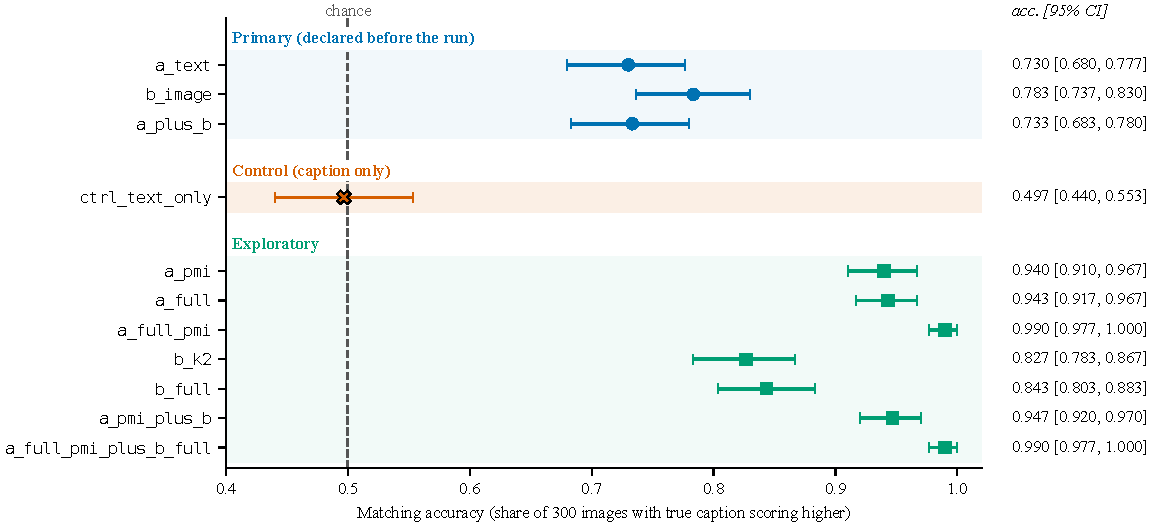
\includegraphics[width=0.92\linewidth]{figures/F1_probe1_accuracy.pdf}
\caption{Matching accuracy of UniDisc 1.4B on true versus mismatched COCO captions (exploratory feasibility result, 300 images).
Markers show the share of images for which the true caption scores higher (chance 0.5, dashed); bars are 95\,\% bootstrap intervals
over images (10\,000 resamples). Blue: primary scores, text direction a\_text and image direction b\_image with $K=8$ complementary
masks, and their sum. Orange: caption-only control, which stays at chance. Green: variants chosen after the primary results (image-masked
null subtracted, single full-mask pass, $K=2$, sums). One run, one mismatch draw; the intervals do not cover variation across draws or
models.}
\label{fig:probe1}
\end{figure}

\subsection{Hardware, runtime and missing items}\label{ssec:hardware}
% run: P2-PROBE-01
All runs use one laptop GPU (NVIDIA RTX 5070 Ti Laptop, 12~GB) with 31~GB of system memory and no other hardware.
In the pilot, one item cost 58 network passes, the median item time was 7.0~s, and the peak GPU memory was 8.2~GB, which is why
passes are batched four rows at a time.
Runs go in short checkpointed chunks under a guard that stops on memory, temperature and power-source events and is resumable;
an abort ends the stage and is not retried until reviewed.
An earlier detection pilot stopped after 20 complete items when the GPU session failed.
% run: P2-PROBE-02
Missing items are handled by a fixed rule: complete cases per analysis, no replacements and no reordering, so that a crash leaves a
prefix of the item list; if the completed base fold has fewer than 240 items, the paper says that the fold is under 80\,\% complete,
prints the minimum detectable effect at the achieved $n$, and does not read ``not rejected'' as evidence against GATE-M.
No analysis that computes $Y$, $b$, $c$, $p$ or a difference of $d_R$ is run on test data before the planned fold is complete.
Mask-seed and corruption-seed variance are not in the intervals, which is a stated limitation.

\subsection{Preregistration, pins and disclosed deviations}\label{ssec:prereg}
The code, the tests, the fold file and the analysis plan are pinned: the code at commit \texttt{164a18a5}, the analysis plan by SHA-256
(\texttt{b4e0bf57...6c47}), and the denoiser check, crash diagnosis and audit files by hash in the repository.
Changes after the pin are logged as amendments; none is made inside a stage.
One analysis preceded the analysis plan and is disclosed.
% run: P2-GATE-CPU/m1_fallback
The first 21 items of the detection set were analysed on CPU before the plan's second addendum, without the gate statistic $q$ (which needs a
GPU pass).
In that exploratory look the mean per-item AUROC against changed-code labels of plain-$B$ was 0.54 on JPEG quality 10 and 0.51 on noise
0.10, while pixel variance with its sign flipped scored 0.76 and 0.77.
The sign of the pixel-variance rival therefore cannot be claimed to be fixed blind, which is why both signs of every rival are admitted
and the rival is chosen on the data.
Any change to the score, $K$, $\alpha$, folds, rungs, arms, family or rival rule that was made after that look and is not a new version of
the preregistration is listed in the change log of the preregistration card and disclosed here.
\todo{AUTHOR: final list of amendments and the date of the first M2 outcome; confirm the status of the open decisions on guard
thresholds, the JPEG denoiser setting and the fallback before the run.}


\section{Results}\label{sec:results}
% results.tex -- card v4 order: the preregistered primary family first, then the secondary families, then the exploratory material.
% Only the detection subsection (run P2-GATE-M1, decision D0074) has data. Every other placeholder names the run directory and the
% wording rule that applies, so that nothing is written beyond what the preregistration allows.
% Each number entered later needs a LaTeX comment "% run: <exp-id>" on the same line or paragraph.

\todo{RESULT: this section is filled only from the frozen run directories after the planned folds are complete. Lead each
subsection with the observation, then the interval, then the preregistered wording from Section~\ref{ssec:tests}. Print the metric
direction in every table header. Every family is reported as run or not run (status map at the end of the section); a family that
was cut is not replaced.}

\subsection{Headroom and operating points}\label{ssec:res_headroom}
\todo{RESULT (run P2-GATE-M3): table of the headroom check, per corruption and rung: $n_v$, $T_1$, $T_2$, pass or fail, the chosen
operating point, $D_c$, $D^\ast$ and the rule (R1, R2 or R3) with the test-fold size. State which corruptions have no operating point
and what that means for the primary family. If no corruption has an operating point, say that the downstream claim is withdrawn.}

\subsection{Calibration of the gate}\label{ssec:res_cal}
\todo{RESULT (runs P2-GATE-M2, P2-GATE-M4 clean arm): realised false-alarm proportion $\hat F$ with item-clustered interval for
$\alpha=0.01,0.05,0.10$; $Z_{\rm cal}$ and the verdict (``no evidence of violation'' or violation); precision among flagged tokens per
corruption; false-alarm proportion on the clean tokens of corrupted items; spatial map of clean false alarms (figure); the exploratory
2\,000-split check of the marginal statement.}

\subsection{Primary result: GATE-M against no gate (family P)}\label{ssec:res_primary}
\todo{RESULT (run P2-GATE-M4): complete Table~\ref{tab:res_primary}; the sentence that applies from the outcome book (SAP Addendum A4,
Part 2) for the label that the committed files give; $n_d$ and, for a null, the statement ``only $\theta\ge\theta^\ast$ would have been
detectable'' (a sensitivity statement, not an observed power). The summary figure shows family P only, with the 90\,\% and 95\,\%
intervals and the lines at $\pm0.05$; the positive control never shares its canvas.}

\begin{table}[t]
\centering
\caption{Primary family: GATE-M versus no gate, paired correctness of the image-direction statistic (higher is better).
\todo{RESULT: test fold size, rule, interval type.}}
\label{tab:res_primary}
\footnotesize
\setlength{\tabcolsep}{2pt}
\begin{tabular}{lccccccc}
\toprule
Corruption (rung) & $n$ & Acc. none & Acc. GATE-M & $b$ / $c$ & $(b-c)/n$ [95\,\%] & $p$ & $p_{\rm Holm}$ \\
\midrule
JPEG & \todo{R} & \todo{R} & \todo{R} & \todo{R} & \todo{R} & \todo{R} & \todo{R} \\
Gaussian noise & \todo{R} & \todo{R} & \todo{R} & \todo{R} & \todo{R} & \todo{R} & \todo{R} \\
Pixel splice & \todo{R} & \todo{R} & \todo{R} & \todo{R} & \todo{R} & \todo{R} & \todo{R} \\
\bottomrule
\end{tabular}
\end{table}

\subsection{Mechanism controls (family S-M)}\label{ssec:res_mech}
\todo{RESULT: GATE-M against the geometry-matched random gate (seed 1 confirmatory; seeds 2 and 3 as replications), the scattered random
gate, plain-$B$ top-$k$ and $s_3$ top-$k$ (counts $b$, $c$ beside the primary result, especially under rule R3), the changed-code gate,
and GATE on clean images. Use the wording of the mechanism rule: if the mechanism test is not rejected, the improvement is ``not
distinguishable from masking the same shape elsewhere, and therefore not attributable to detection beyond mask geometry''.}

\subsection{Detection against cheap rivals (family S-D)}\label{ssec:res_det}
% run: P2-GATE-M1
This family was analysed before the main test, on the 200 detection items, and it is a measurement of the within-modality score $q$;
it enters no claim about the primary result.
Intervals are 95\,\% percentile bootstrap intervals over items for the per-item AUROC against changed-code labels; items with too
few corrupted or clean tokens are excluded and counted (3 for JPEG, 2 for noise).
On the sanity corruptions $q$ reaches 0.961 (0.959 to 0.963) for a replaced patch and 0.955 (0.952 to 0.957) for swapped codes, so the
chance bar of the positive control was passed; plain-$B$ is slightly higher, 0.964 and 0.960, with $q$ minus plain-$B$ equal to
$-0.0033$ ($-0.0042$ to $-0.0026$) and $-0.0053$ ($-0.0058$ to $-0.0047$).
The non-finetuned TbV score reaches 0.854 and 0.859 and the neighbour codebook distance 0.786 and 0.741 on the same corruptions; a
check for copying of the released output layer suspected no item.
On JPEG quality 10 $q$ reaches 0.561 (0.547 to 0.575, 197 items) and on Gaussian noise 0.10 it reaches 0.503 (0.493 to 0.513, 198
items).
The non-finetuned TbV score reaches 0.581 (0.569 to 0.593) on JPEG and 0.607 (0.597 to 0.618) on noise; on noise the marginal
intervals of $q$ and TbV do not overlap, on JPEG they do, and no paired test between them was run.
The best cheap rival is the pixel variance of a token's patch with its sign flipped, 0.756 (0.743 to 0.768) on JPEG and 0.768 (0.760
to 0.776) on noise.
The rival and its sign were chosen on the data among about nine candidates, which biases the contrast against $q$.
The paired difference of $q$ minus the rival is $-0.195$ ($-0.214$ to $-0.175$) on JPEG and $-0.265$ ($-0.278$ to $-0.253$) on noise,
with a Holm-adjusted $p$ of 0.0004 on each, the resolution floor of 10\,000 resamples.
The result is the same when the rival is re-selected in every resample and when the 21 items analysed before the plan's second
addendum are removed (179 items).
The preregistered falsifier for the score was therefore met on both corruptions, and the paper does not say that the score detects
corrupted codes better than cheap methods.
That a texture score wins against this label is read as the label-circularity concern of Section~\ref{ssec:limits} and not as
evidence that texture explains the corruption effect.
\todo{RESULT (runs P2-GATE-M4, family S-D2): the same contrast on the test items at their operating points, including splice if it has
one; the detection of splice has not been measured outside the main run.}

\subsection{Positive control (family PS)}\label{ssec:res_ps}
\todo{RESULT (run P2-GATE-M4, patch and swap): the table of the same test as the primary family, Holm over two, in its own table and
never beside the primary rows. Wording: ``the pipeline is not broken'' if both are rejected with $b>c$, ``pipeline defect suspected,
audit triggered'' otherwise. Nothing is said about where the gate works.}

\subsection{Pixel denoising as a defence (family S-DN)}\label{ssec:res_dn}
\todo{RESULT: GATE-M against the denoised copy on JPEG and noise; for JPEG use the wording that the denoiser harms the image at this
setting.}

\subsection{Evidence ratio and sign agreement of the independent-token calculation (families S-Z and E-pred)}\label{ssec:res_snr}
\todo{RESULT: paired change of $d_R$ (and $z_R$ as sensitivity) per corruption. For E-pred: the plug-in estimates of
$\rho,\mu,\sigma^2,\mu_c,\sigma_c^2,\hat\phi_0,\hat\phi_1$ from the per-token terms, and the sentence ``the sign of the plug-in
signal-to-noise change agreed with the sign of the net accuracy difference in $A$ of $K_{\rm eval}$ cells'' with its interval, P and PS
cells separate and both signs shown. The word ``predicted'' is used only inside the E-pred table columns.}

\subsection{Decomposition of the accuracy lost to corruption (descriptive, E-dec)}\label{ssec:res_edec}
\todo{RESULT: the residual loss under the changed-code gate and the gap to that gate, with paired bootstrap intervals. No test and no use
of these parts as an account of the primary result.}

\subsection{Coherence of the denoiser across mask patterns}\label{ssec:res_coh}
\todo{RESULT: the median absolute gap against the 95th percentile of the repeat gap, and the pre-stated reading.}

\subsection{Re-infilling the flagged tokens (family S2)}\label{ssec:res_s2}
\todo{RESULT (run P2-GATE-S2, or ``not run'' with the reason): patch and splice, I-GATE against I-RAND4 (kept draw) with the draw-level
and all-four contrasts beside it, I-GATE against none printed beside it, completed $n$ and whether it is a partial prefix. The claim-bearing
cell is splice; a patch-only rejection is a positive control with no realistic cell. No statement for JPEG or noise, and the string
``G.1'' is not used.}

\subsection{Two-way fusion on hard negatives (family B)}\label{ssec:res_text}
\todo{RESULT (run P2-GATE-FOIL, or ``not run''/``untestable at ceiling'' with the clean accuracy of the better single direction): fusion
against the better single direction, the two margins and the frozen fusion line. Text-direction conditioning arms for the three
realistic corruptions with intervals (exploratory).}

\subsection{Second model (family R)}\label{ssec:res_omni}
\todo{RESULT (runs P2-OMNI-R-TEST, or ``not run: no rejection with $b>c$ in P''): directional replication on a second model, 4-bit
quantised, with the confound list and, under rule~R2, the statement that the same test images were used; ``not replicated;
inconclusive at this $n$'' for a non-rejection. Never pooled with UniDisc and never ``generalises''.}

\subsection{Exploratory comparisons}\label{ssec:res_expl}
\todo{RESULT (run P2-GATE-M4, \texttt{tier3\_fusion.json}, or ``not run''): the exploratory comparison of Section~\ref{ssec:tier3} in
its own table, primary-family cells and positive-control cells in separate panels, with the number of intervals, ``no multiplicity
adjustment'', the minimum detectable difference beside every interval, and the four limits printed beside the table. The three-way reading
and the placement rule of the plan apply: nothing here explains, qualifies or rescues a primary result. The exploratory corruption suite
(Appendix table, intervals only) is reported here as well.}

\subsection{Status of every family and cost}\label{ssec:res_cost}
\todo{RESULT: one line per family with its status (run, descriptive, partial prefix, untestable at ceiling, not run with the reason).
Network passes per item by stage, median time per item and peak GPU memory, from the run configuration and telemetry files.}


\section{Discussion and limitations}\label{sec:discussion}
% discussion.tex -- Findings written 2026-10-29 for the label NEG of P (SAP Addendum A4, A4.2.3: opening of 6.1 near-verbatim).
% The fusion-context and limitations subsections are outcome-independent and drafted from the preregistration (card v4, SAP, A4).
% No sentence in this file draws on PS, S2, B, R, E-dec, E-pred, the suite, detection or the exploratory comparison to explain, qualify
% or predict the primary result (AB.1). The phrase "when does input gating help" is not used (D18 reading 1, decisions D0076-D0077);
% after the opening, the question of when gating can help is discussed only through the closed-form condition and the P table.
% Proposition 2 (correlated tokens) is not used on E-pred (D0078); Proposition 1 of the theory addendum is not used (D0078-D0079).

\subsection{Findings}\label{ssec:disc_findings}
% run: P2-GATE-M4 (analysis.json primary.*)
The preregistered test excludes an improvement or a loss of more than five percentage points in image-direction verification accuracy
from gating under JPEG quality~10, Gaussian noise with $\sigma=0.10$ and a $128$-pixel splice, for this model and these severities; it
does not show that gating has no effect.

The primary table shows how narrow the measured change is: in 500 items the gate changed the decision once under JPEG, never under
noise and four times under splice (Table~\ref{tab:res_primary}).
The exclusion of $\pm0.05$ is a statement about these discordances at the threshold calibrated for $\alpha=0.05$, at one severity per
corruption, in one model and on one data set.
It says nothing about a gate that flags a larger share of tokens, about stronger corruptions, or about another model or task, none of
which was tested.
Section~\ref{ssec:evidence} gives, under independent tokens, the condition on the hit and false-alarm rates under which discarding
flagged tokens raises the signal-to-noise ratio of an additive evidence sum (Eq.~\eqref{eq:snr}).
The condition states what a gate would have to achieve; it is an approximation for dependent image tokens, the test was not designed to
check it, and we do not use it to account for the result.

The remaining findings are separate measurements, each under its own family label, and none of them is an account of the primary result.
For each we give the observation, a hypothesis for it, and what would falsify the hypothesis.

\emph{The clean false-alarm statement held; the flags on corrupted images are not covered by it.}
% run: P2-GATE-M4 (calibration.*)
On held-out clean pairs the realised flagged share was 0.0456 at $\alpha=0.05$ (95\,\% interval 0.0442 to 0.0470), with no evidence
of violation at any of the three levels (Section~\ref{ssec:res_cal}).
On the unchanged tokens of corrupted images the false-alarm proportion was 0.036 to 0.044 for the realistic corruptions and 0.089 under
swap, above $\alpha$.
The conformal statement covers clean pairs only, so these proportions lie outside it; the audit of the positive control
did not treat the 0.089 as a defect for that reason.
Hypothesis: a token next to a replaced code is scored with damaged context and is flagged more often, as Section~\ref{ssec:calibration}
anticipates.
It would be falsified if, under swap, the false-alarm proportion of an unchanged token did not fall with its distance to the nearest
replaced code; this was not measured.

\emph{The gate's score was near chance at finding the codes that JPEG and noise change.}
% run: P2-GATE-M1; P2-GATE-M4 (s_d2.*, calibration.per_condition.*)
On the detection items and again on the test items (families S-D and S-D2) the per-item AUROC of $q$ was 0.561 under JPEG and 0.503 and
0.509 under noise, below a texture score whose sign was chosen on the data; under noise the hit rate of the gate (0.033) was below its
false-alarm proportion on unchanged tokens (0.036).
Hypothesis, the label-circularity concern of Section~\ref{ssec:limits}: JPEG quality~10 and noise change more than nine in ten codes of
an image (Table~\ref{tab:res_flags}), so a changed code marks where the tokenizer is unstable more than where the image is damaged, and a
texture score tracks that instability.
It would be falsified if $q$ stayed at chance against a damage label defined in the pixel domain, for example the reconstruction error
of each token's patch, under which texture had no advantage; this was not measured.

\emph{A pixel denoiser restored most of the accuracy lost to noise.}
% run: P2-GATE-M4 (s_dn.*, c1_test.accuracy)
Under noise the denoised copy reached 0.852 against 0.676 without a gate and 0.880 on clean images, and it gave higher verification
accuracy than GATE-M (family S-DN, Section~\ref{ssec:res_dn}); under JPEG no difference was detected, with a denoiser setting that
lowers JPEG image quality.
Hypothesis: noise of this strength is largely removed in the pixel domain before tokenisation, so the tokens of the denoised image are
close to the clean ones.
It would be falsified if the share of codes that differ from the clean tokenisation were not lower for the denoised noisy images than for
the noisy ones; this was not measured.
The denoiser is a measured comparator, not part of the gate, and one setting was used.

\emph{Withholding every changed code lowered accuracy under JPEG.}
% run: P2-GATE-M4 (mechanism.jpeg10.y.changed_code_minus_none; edec.json cells.P1; calibration.per_condition.jpeg10.prop4.rho)
The changed-code gate, which keeps only the codes that the corruption left unchanged, lowered accuracy under JPEG by 0.084 and raised it
under noise by 0.070 (Table~\ref{tab:res_mech}); in E-dec the gap to this oracle was negative under JPEG with an interval that excludes
zero, which by the plan voids any detection reading of that cell (Section~\ref{ssec:res_edec}).
Hypothesis: under JPEG this gate decides on about four percent of the tokens of an image, and the sum over so few tokens is noisier than
the sum over all of them, which is the composition effect named in the plan.
It would be falsified if keeping a random set of the same small size, instead of the unchanged codes, did not lower accuracy by a similar
amount; this was not measured.

\emph{Exploratory: no detector-free combiner was above the hard gate on a realistic corruption.}
% run: P2-GATE-M4 (tier3_fusion.json)
In the exploratory comparison (Section~\ref{ssec:res_expl}; Tier~3, intervals only), the hard gate gave higher verification accuracy
than the median and the 20\,\% trimmed mean under JPEG and splice; the data do not show a difference between the hard gate and the
trimmed mean at the gate's flag count on any realistic corruption, nor between the hard gate and the median or the 20\,\% trimmed mean
under noise, with bounds at most 0.05, which counts by the pre-stated rule as a finding against the added value of the detector on those
cells.
Discarding the flagged tokens and discounting or weighting them were not distinguishable on any realistic corruption.
This is a property of these combiners on these cells, measured on the same evidence as the primary test, and not an account of the
primary result; when the gate's score is near chance, the comparison with the trimmed mean at the gate's flag count largely repeats the
primary contrast (limit (c) of Table~\ref{tab:res_tier3}).

\emph{The positive control was not met; the audit it triggered found no defect.}
% run: P2-GATE-M4 (ps.*); P2-A23-AUDIT
On the two sanity corruptions the gate did not change accuracy detectably (Section~\ref{ssec:res_ps}): positive control not met; audit
triggered (SAP A2.3); no defect found, with $n_d=4$ (patch) and $n_d=13$ (swap) discordant items.
The audit covers the classes of error that the plan names and does not validate the pipeline; Section~\ref{ssec:res_ps} states what
it cannot see.
Nothing in the positive control is used in this paper to account for the primary result.

\emph{Post hoc and descriptive: the decision headroom of the positive control.}
% run: P2-A23-AUDIT (a23_ps_audit.json, per_condition.{patch,swap}); P2-GATE-M4 (ps.*)
This paragraph was written after the outcome of PS was known, enters no test, and describes the task and the design of PS, not the
gate.
Without a gate, the sanity corruptions changed the decision on 5 of the 500 test items under patch (all five from right to wrong) and
on 9 under swap (7 from right to wrong, 2 from wrong to right), that is on 0.010 and 0.018 of the items.
With no losses, the exact two-sided McNemar test at the first Holm step (level 0.025) needs at least 7 wins; a gate that returned every
item to its decision on the clean image would have given $b=5$, $c=0$, $p=0.0625$ under patch and $b=7$, $c=2$, $p=0.18$ under swap,
and would not have reached that step.
The changed-code arm, which uses the true set of replaced codes, did not either ($b=4$, $c=2$, $p=0.69$ under patch; $b=7$, $c=4$,
$p=0.55$ under swap), and GATE-M made the same decision as that arm on 498 of the 500 items in each cell.
The discordance between GATE-M and no gate was 0.008 under patch and 0.026 under swap, against the 0.05 to 0.20 that the power
calculation of the plan assumed (AD.4, where it is marked as an assumption).
At that discordance this test could not have rejected for a perfect gate, so the positive control, as designed, cannot separate a
working pipeline from a broken one on these two corruptions; this is a property of the task, where replacing 64 or 154 codes rarely
turns a correct decision into a wrong one, and of the design, which assumed more discordance than occurred, and not a statement about
the method.
The description is not used to account for the primary result, and the positive control is not read as met on this ground.

\subsection{Where the work sits in information fusion}\label{ssec:disc_fit}
\emph{What is fused.}
The 1\,024 image tokens of one image are 1\,024 sources.
Each reports a log-likelihood ratio between two candidate captions, and the decision sums them; a second, text-direction statistic can
be fused with that sum at score level (family B).
\emph{At what level.}
At the input: the gate acts on the sources before the evidence sum, not on the output decision, which is why the paper speaks of
input-level source validation.
\emph{Where reliability enters.}
Only through a zero-one weight in the sum (GATE-M) or through replacement of the flagged values by a model draw (GATE-I).
The weight is computed from within-modality evidence alone, and its threshold is set on clean data at a fixed false-alarm level, as in
CFAR detection.
\emph{What is not claimed.}
The paper claims no new fusion rule.
The additive rule is optimal only for sources that are independent given the hypothesis, which image tokens are not, and the hard
weight is not claimed to be the best way to use a reliability estimate; graded weights and robust aggregation are the standard
alternatives, and Section~\ref{ssec:tier3} states the exploratory comparison with them.

The calibrated gate of Zhou and Lu~\cite{zhou2027burden} and the gate studied here answer different questions.
As described in the abstract of Zhou and Lu, theirs decides which of two recognisers to believe for one test instance; the gate
here decides which input tokens to withhold before two directions of image-text evidence are combined.
The two could be stacked, but this is not tested.
Evidential fusion~\cite{shao2024ddef,huang2025evidential} and conformal prediction sets on a fusion network~\cite{wang2025multistage}
are other uses of reliability and of distribution-free calibration in this journal that we found; as far as their abstracts describe,
none scores input tokens with the likelihood of a generative model.
\todo{AUTHOR: after the results are frozen, give the abstract and Figure~1 caption to a reader with no project context and ask what is
fused (open check on the scope-fit question); settle the scope-fit question with the supervising professor before submission.}

\subsection{Limitations}\label{ssec:limits}
Except for the two items on the positive control, the limitations below are fixed by the design and do not depend on the outcome.
\begin{itemize}
\item \emph{One model, one data set.} All measurements of the primary family use UniDisc 1.4B and COCO val2017 images as tokenised
by one tokenizer. A second, 4-bit quantised model was to enter only in family R, only if P had a rejection with $b>c$; P had none, so R
was not run. No statement is made for other models, resolutions, caption styles or data sets.
\item \emph{Contamination is unknown.} Whether the evaluation images were in the training data of the model or of the tokenizer was not
established, and it could make clean pairs easier than unseen ones. The same applies, with more force, to the hard-negative set,
whose true captions are COCO captions.
\item \emph{Narrow guarantee.} The calibration bounds the expected false-alarm proportion on clean, exchangeable test pairs. It gives
no bound on detection power, none on the clean tokens of corrupted items, and none under shift. Unlike a selective-risk bound on
the harm of an action, as described for Zhou and Lu~\cite{zhou2027burden}, it says nothing about the harm or the power of the gate
on corrupted inputs. The realised proportion on one finite test set can lie above $\alpha$ because the statement is marginal over the
calibration draw.
\item \emph{Corruptions and labels.} Corruption labels are relative to the tokenisation of the clean image, so a ``clean'' token
may already carry compression artefacts of the original photograph. Changed codes under JPEG and noise concentrate where the tokenizer
is unstable, so the label may track tokenizer instability more than damage: a texture rival that wins against this label is not
thereby shown to explain the corruption effect, and the changed-code gate is not an upper bound for these corruptions.
\item \emph{Comparators chosen on the data.} The best cheap rival is selected among about nine candidates, with both signs admitted, which
biases the detection contrast against the gate. The rival's sign could not be fixed blind (Section~\ref{ssec:prereg}).
\item \emph{Pixel denoiser.} One setting was used for all corruptions; it was chosen after one exploratory evaluation on 20 images and
harms JPEG images, so the denoising contrast on JPEG favours the gate.
\item \emph{Variance not in the intervals.} Intervals cover item sampling. They do not cover variation across mask partitions, corruption
draws, jitter seeds or models, because no training seeds exist and only one corruption draw is made per image. Eleven test families
are run with no multiplicity control across them.
\item \emph{A constructed task.} The primary decision is a two-way caption match on the weaker of the two available statistics, with
random negatives (Section~\ref{ssec:task}). It measures how an image-direction statistic tolerates damage and says nothing about
what a gate adds to a verifier that uses the stronger text direction; only family B addresses the two-direction setting, and it may be
untestable at the ceiling or not run.
\item \emph{A hard gate and dependent tokens.} The gate is binary, and the evidence sum and the signal-to-noise analysis assume
independent tokens, which neighbouring image tokens are not. Graded and robust alternatives are examined only in an exploratory
comparison (Section~\ref{ssec:tier3}), which is not a test and is subject to its own limits.
\item \emph{Time input and checkpoint.} The scorer calls the denoiser without a time input; that this is the intended path was checked
for the released configuration and checkpoint only, the training weight of whole-modality masks is unknown, and the key check does not
cover the image tokeniser (Section~\ref{ssec:data}, \ref{app:timefree}).
\item \emph{Scope of the preregistered run.} Families S2 (re-infilling), B (two-way fusion) and R (second model) each have a status of
run or not run, decided by time and by their gatekeeping rule and never by an outcome, and the paper reports that status.
Caption corruption, the backbone authors' own re-infill recipe and the gating of caption tokens are not tested as families.
\item \emph{Positive control not met.} The preregistered positive control on the sanity corruptions was not met, which triggered a
pipeline audit (Section~\ref{ssec:res_ps}); the audit found no defect. It was run after the outcome was known and covers the classes
of error that the plan names. A recomputation from the stored arrays cannot see an error upstream of them, and the audit does not
validate the pipeline. The conformal statement covers clean pairs only; on the unchanged tokens of swapped images the flag proportion
was 0.089, above $\alpha$, which the audit recorded and did not count as a defect.
\item \emph{Power assumption of the positive control.} The plan's power calculation for the positive control assumed a discordance of
0.05 to 0.20 between the gated and the ungated decision. The realised values were 0.008 and 0.026 ($n_d=4$ and 13 of 500), and at
that headroom the preregistered test could not have rejected even for a gate that restored every clean decision. The positive control
therefore cannot separate a working pipeline from a broken one on these two corruptions. This is a property of the design and of the
task, not of the method, and it is not used to account for the primary result.
\item \emph{Hardware and missing data.} The GPU is a single laptop device that failed in earlier pilots. A crash leaves a prefix of the item
list and the missing-item rule applies; a fold under 240 items is reported as incomplete.
\item \emph{Narrow novelty.} Detecting and remasking corrupted input tokens, cross-modal remasking, risk-controlled thresholds for
vision-language errors, including gates that decide between whole predictions~\cite{zhou2027burden}, and masked-likelihood scores
each have precedents (Section~\ref{sec:related}). The claim is a measurement of their composition on one model, and it holds only as
far as the measured results go.
\item \emph{Concurrent work.} A search for concurrent work was last run on 28 October 2026; unpublished or under-review work is not
visible, and the closest paper in this journal~\cite{zhou2027burden} was compared from its abstract and preview only.
\todo{AUTHOR: repeat the search once before submission, and read the full text of Zhou and Lu.}
\end{itemize}


\section{Conclusion}\label{sec:conclusion}
% conclusion.tex -- 3 to 5 sentences, same numbers as the paper, limits in one sentence, future work in one sentence, no new claim.
% Placeholders only: no result exists.

\todo{RESULT, sentence 1: the question and the measurement, stated as in the contribution paragraph, scoped to one pretrained model and one data set.}

\todo{RESULT, sentence 2: the headroom outcome and the primary contrast per corruption, with the number, interval and preregistered wording.}

\todo{RESULT, sentence 3: the calibration result (realised false-alarm proportion and the verdict) and the mechanism and detection controls.}

\todo{RESULT, sentence 4: limits in one sentence (one model, one data set, narrow guarantee, no re-infill or caption corruption in the main run).}

\todo{AUTHOR, sentence 5: future work in one sentence (a second backbone; the re-infill and caption-corruption tiers; a finetuned variant of the observed-position score).}


% declarations.tex -- order follows the Information Fusion exemplar and the Guide for Authors: CRediT, generative-AI declaration,
% competing interests, funding, acknowledgements, data availability, then the reference list (added in main.tex).
% Per Shlok's decision, AI use is described ONLY in the section "Declaration of generative AI ..." below, and nowhere else.

\section*{CRediT authorship contribution statement}
\textbf{Shlok Kumar Goenka:} \todo{AUTHOR: choose from the 14 CRediT roles (conceptualization, methodology, software, validation, formal analysis, investigation, data curation, writing -- original draft, writing -- review and editing, visualization, ...)}.
\textbf{\todo{AUTHOR: supervising professor}:} \todo{AUTHOR: roles (for example supervision, project administration, writing -- review and editing)}.

\section*{Declaration of generative AI and AI-assisted technologies in the manuscript preparation process}
\todo{AUTHOR (Shlok): exact wording of this declaration. The Elsevier template sentence is: ``During the preparation of this work the author(s)
used [NAME OF TOOL/SERVICE] to [REASON]. After using this tool/service, the author(s) reviewed and edited the content as needed and take(s)
full responsibility for the content of the published article.'' Name each tool, its version and its purpose, and the extent of review.
Decision still open for Shlok: whether any AI-assisted step of the research process (code, analysis) must also appear in the methods under the
journal's policy; the project rule keeps every AI mention in this section.}

\section*{Declaration of competing interest}
\todo{AUTHOR: complete the Elsevier declarations tool and state ``The authors declare that they have no known competing financial interests or personal relationships that could have appeared to influence the work reported in this paper'' only if true.}

\section*{Funding}
\todo{AUTHOR: funding sentence. If there is none, the fixed Elsevier sentence is ``This research did not receive any specific grant from funding agencies in the public, commercial, or not-for-profit sectors.''}

\section*{Acknowledgements}
\todo{AUTHOR: acknowledgements, if any.}

\section*{Data availability}
% Option C of the journal: research data, code and scripts are deposited in a repository and linked.
\todo{AUTHOR: repository and DOI. Planned content: the code at commit \texttt{164a18a5} (\texttt{exp\_p2/}, \texttt{tests/exp\_p2/}), the fold file
(SHA-256 \texttt{\seqsplit{450edb543779de7ee5e6a52422fd6507ef52f15ba3b956a8b05c2e561620f311}}), the preregistration card, the analysis plan (SHA-256
\texttt{\seqsplit{b4e0bf575dfc2524c0f9d3d5c6b5f52e3185088a94ced8c75f092104ed396c47}}), per-item scores and predictions of every run directory cited,
the analysis and figure scripts, and the licence. The COCO images and captions and the UniDisc and tokenizer weights are third-party and are cited, not redistributed.
Do not write ``available on request''.}


\bibliographystyle{elsarticle-num}
\bibliography{references}

\end{document}
